\documentclass[12pt]{article}

\usepackage[utf8]{inputenc}
\usepackage{amsmath}
\usepackage{graphicx}
\usepackage[hidelinks]{hyperref}
\title{RefonteSousSymfony}
\author{Faiza Merah}
\date{November 2024}


\begin{document}

    \section*{Remerciements}
    Avant de présenter notre travail, nous tenons à remercier M. Florian LITOT, ingénieur à l’Institut des Sciences et Techniques de l'Antiquité de Besançon, qui nous a proposé le sujet de ce projet et nous a reçus régulièrement durant son développement afin de répondre à nos interrogations et de nous aiguiller durant toute la conception de l’application.
    \newline
    \newline
    Nous sommes également reconnaissants envers l’ensemble de nos professeurs de l’UFR ST de Besançon pour nous avoir donné les connaissances techniques, ainsi que l’organisation autour d’un projet tel que celui-ci. Pour finir, nous remercions nos proches, qui ont été les testeurs de cette application, et dont les retours précieux nous ont permis d’améliorer le visuel et le comportement de notre application.
    \newpage

    \tableofcontents
    \newpage

    \listoffigures
    \newpage

    \section*{Glossaire}

    \begin{itemize}
        \item \textbf{CRUD} : Opérations de base d’une base de données (Create, Read, Update, Delete).
        \item \textbf{DataTable} : Tableau interactif avec tri, recherche et pagination.
        \item \textbf{Debian} : Système d’exploitation Linux stable.
        \item \textbf{Doctrine} : ORM pour gérer les bases de données en PHP.
        \item \textbf{EntityManager} : Gestionnaire d’entités et transactions en Doctrine.
        \item \textbf{Framework} : Environnement de développement (Exemple : Flutter, Symfony, …).
        \item \textbf{MVC}: Modèle-Vue-Controleur
        \item \textbf{JSON} : Format d’échange de données léger et structuré.
        \item \textbf{ORM} : Liaison entre objets et base de données sans SQL direct.
        \item \textbf{Package} : Ensemble de fichiers ou bibliothèques réutilisables.
        \item \textbf{PHP} : Langage de programmation servant notamment à produire des pages web.
        \item \textbf{Route} : Association d’une URL à une action spécifique.
        \item \textbf{Symfony} : Ensemble de composants PHP. Il fournit des fonctionnalités modulables et adaptables qui permettent de faciliter et d’accélérer le développement d'un site web.
        \item \textbf{Twig} : Moteur de templates pour PHP et Symfony.
    \end{itemize}

    \newpage


    \section{Introduction}
    Symfony est un framework PHP d’origine française, qui permet de développer des applications web tout en évitant de recréer des fonctionnalités courantes telles que la gestion des utilisateurs ou des routes. Grâce à son architecture modulaire et à son écosystème riche, Symfony offre aux développeurs des outils performants pour concevoir des applications complexes.
    \\
    \\
    Un projet tel que celui-ci peut s’avérer exigeant, notamment en raison du nombre croissant de routes à gérer et des données à manipuler. Dans ce contexte, un outil comme Symfony se révèle essentiel pour gagner du temps et optimiser les efforts de développement tout en garantissant une structure robuste et évolutive.
    \\
    \\
    Dans le cadre de notre deuxième année de Master ISL à l’Université Marie et Louis Pasteur, nous avons réalisé ce projet de développement web entre octobre 2024 et février 2025, sous la supervision de M. Florian Litot. Ce projet a été l’occasion de mettre en pratique nos compétences en développement web, tout en approfondissant nos connaissances en conception logicielle et en gestion de bases de données relationnelles.
    \\
    \\
    Ce rapport vise à présenter en détail les différentes étapes du développement de notre application. Dans chaque partie, nous décrirons le sujet abordé, mais également les difficultés que nous avons rencontrées durant celle-ci.
    \\
    Dans un premier temps,nous parlerons de la première étape que nous avons traversée, la migration des versions de Symfony.
    \\
    Ensuite, nous décrirons les fonctionnalités principales de l'application, ainsi que les différents rôles pouvant être attribués aux utilisateurs.
    \\
    Après cela, nous expliquerons l'architecture de l'application et comment nous faisons les liaisons avec la base de données.
    \\
    Nous aborderons ensuite la façon dont nous nous sommes organisés durant la totalité de ce projet, à la fois pour la répartition du travail mais également pour la communication entre nous.
    \\
    Enfin, nous verrons les résultats que nous avons obtenus, et que l'on comparera aux points attendus lors du début du projet.

    \newpage


    \section{Présentation du projet}

    Le laboratoire ISTA (Institut des Sciences de l’Antiquité), spécialisé dans l’étude des sociétés anciennes et des recherches sur l’esclavage, dispose d’un site web destiné à centraliser et exploiter ses données scientifiques. Dans le cadre de ce projet, le site a été modernisé et adapté aux besoins actuels à l’aide du framework Symfony.
    \newline
    L’objectif principal de ce projet est de fournir une plateforme optimisée pour la gestion et l’exploitation des données du laboratoire. Le site intègre des outils permettant d’effectuer des recherches avancées, d’exporter les résultats dans différents formats (Word, PDF, Excel) et de visualiser les données sous forme de statistiques claires et accessibles.
    \newline
    Ce projet a été conçu pour s’intégrer parfaitement à la base de données existante et pour fonctionner sur un environnement Debian 10, assurant une compatibilité optimale et une transition fluide vers une solution technologique moderne, adaptée aux exigences des chercheurs et des utilisateurs.


    \section{Migration vers Symfony 7}

    \subsection{Raisons de la migration}
    - Raisons techniques (performance, nouvelles fonctionnalités de Symfony 7).
    - Compatibilité avec les versions modernes de PHP et des dépendances.

    La migration de l'application de Symfony 6.3 vers Symfony 7.1, la dernière version stable, a été effectuée afin de tirer parti des améliorations de sécurité, des nouvelles fonctionnalités et des performances optimisées. Opter pour la dernière version permet de rester à jour, d'assurer la compatibilité et de réduire les risques liés aux anciennes versions.

    \subsection{Préparation à la migration}
    Avant de démarrer la migration, nous avons procédé comme suit:
    \begin{itemize}
        \item Un audit de compatibilité a été effectué pour analyser toutes les dépendances de l'application et identifier les éventuelles incompatibilités.
        \item Les dépréciations liées à la version 6.3 ont été relevées et corrigées en utilisant les outils fournis par Symfony.
        \item Nous avons étudié attentivement le guide de mise à jour de Symfony pour comprendre les étapes et ajustements nécessaires.
    \end{itemize}

    \subsection{Étapes de la migration}
    \begin{itemize}
        \item \textbf{Migration progressive via les versions intermédiaires}:
        Selon la documentation officielle, il est recommandé de ne pas effectuer de saut direct entre deux versions majeures. Nous avons suivi un chemin de migration progressif, en passant par les versions mineures. Ainsi, nous avons d'abord migré vers la dernière version mineure de la série 6.3, puis vers 6.4 puis vers première version majeure de la série 7.x, et enfin vers la version 7.1.

        Cette approche garantit une transition stable, car les versions mineures incluent des outils de déprécations permettant d'adapter le code avant de passer à une version majeure.
        \item \textbf{Mise à jour des dépendances}: À chaque étape, nous avons mis à jour les bibliothèques et packages liés à Symfony. Un effort particulier a été fait pour vérifier la compatibilité de toutes les dépendances avec la nouvelle version.
        \item \textbf{Gestion des dépréciations}:Les fonctionnalités obsolètes identifiées lors de l’audit ont été remplacées ou ajustées conformément aux recommandations. Les fichiers de configuration, les contrôleurs et les services ont été adaptés aux nouvelles normes de Symfony
    \end{itemize}

    \subsection{Problèmes rencontrés et solutions apportées}
    - Exemple : erreurs liées à des dépendances obsolètes.

    Après la migration vers Symfony 7, certains morceaux de code obsolètes ou incompatibles ne fonctionnent plus correctement. Par conséquent, des changements dans le code sont nécessaires pour assurer le bon fonctionnement de l’application. Voici un exemple concret de problème rencontré :
    \begin{itemize}
        \item \textbf{Problème des séquences d'ID} : Avant la migration, la stratégie `IDENTITY` était utilisée par défaut, mais cela a généré l'erreur dans la figure \ref{fig:warning1} :
        \begin{figure}[h]
            \centering
            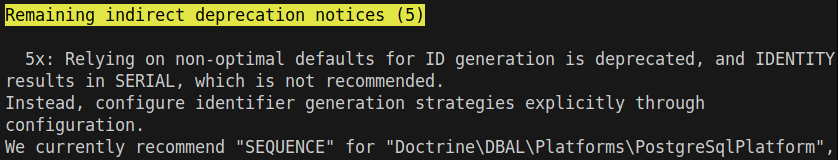
\includegraphics[width=0.8\textwidth]{images/Capture d’écran du 2024-11-16 18-54-54.png}
            \caption{Deprecation notice }
            \label{fig:warning1}
        \end{figure}
        \newpage
        Pour résoudre ce problème, il a fallu remplacer l'annotation \texttt{#[ORM\GeneratedValue]} par \texttt{#[ORM\GeneratedValue(strategy: "SEQUENCE")]} dans toutes les entités, comme recommandé par Symfony.
    \end{itemize}

    \subsection{Validation de la migration à travers les tests}

    Avant de développer de nouvelles fonctionnalités, il est essentiel de vérifier que la migration vers Symfony 7 a été effectuée correctement. Cela permet de s'assurer que l'application fonctionne comme prévu, garantissant ainsi une base stable pour le développement futur.

    Dans cette section, les tests d'intégration réalisés ont permis de vérifier que la migration vers Symfony 7 s'est correctement effectuée (Figure \ref{fig:integration}), en particulier en ce qui concerne la base de données et l'ORM. L'objectif principal de ces tests était de valider la connexion à la base de données et le bon fonctionnement des opérations CRUD. Une base de données dédiée a été utilisée pour éviter toute interférence avec les données de production. Ces tests ont permis de s'assurer que l'EntityManager de Symfony fonctionne correctement avec la base de données, garantissant ainsi que les entités peuvent être créées, mises à jour, lues et supprimées sans erreurs. Les opérations suivantes ont été testées :

    \begin{itemize}
        \item Création d'un utilisateur avec des champs comme `username`, `password`, et `roles`.
        \item Récupération de l'utilisateur depuis la base de données pour vérifier que les données ont été correctement insérées.
        \item Mise à jour d'un utilisateur et vérification que les changements sont bien persistés dans la base.
        \item Suppression d'un utilisateur et vérification que l'entité est supprimée de la base de données.
    \end{itemize}
    \begin{figure}[h]
        \centering
        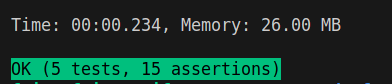
\includegraphics[width=0.6\textwidth]{images/Capture d’écran du 2024-11-16 18-33-01.png }
        \caption{Résultats des tests d'intégration}
        \label{fig:integration}
    \end{figure}


    \section{Fonctionnalitées ajoutées}

    \subsection{Gestion des Autorisations sur les Index}
    Une nouvelle fonctionnalité permet à l'administrateur de gérer les autorisations sur les index via une interface basée sur un DataTable, comme illustré à la figure \ref{fig:gestion_autorisations_index}. Cette interface offre des options de tri, de recherche, et de sélection multiple pour accorder des autorisations à des utilisateurs simples. En conséquence, les utilisateurs simples peuvent modifier ou supprimer (via une suppression sécurisée) uniquement les index pour lesquels ils ont obtenu des autorisations, améliorant ainsi la sécurité et le contrôle d'accès.\\
    \\
    \textit{\textbf{Implémentation Technique:}}
    Pour implémenter cette fonctionnalité, une nouvelle table \textit{index\_auth} a été ajoutée à la base de données pour gérer les autorisations associées aux index. Des fonctions spécifiques ont été créées dans le \textit{IndexController} pour gérer les autorisations, et des vues Twig comme \textit{auth.html.twig} ont été développées pour afficher l'interface utilisateur. \\
    \\
    \textbf{Accès: }
    Pour accéder à cette fonctionnalité : \\
    Côté Administrateur : Naviguer vers Administration $\rightarrow$ Gestion des Index, puis utiliser le bouton Donner Autorisations.\\
    Côté Utilisateur : Accéder à Profil $\rightarrow$ Voir mes Index Autorisés pour voir les index avec des autorisations.

    \subsection{Gestion des Autorisations sur les Livres}
    Cette fonctionnalité permet à l'administrateur de gérer les autorisations des utilisateurs sur les livres comme illustré à la figure \ref{fig:gestion_autorisations_livre}. L'administrateur peut attribuer des droits spécifiques à des utilisateurs simples, leur permettant de modifier ou de supprimer (de manière sécurisée) les livres auxquels ils ont accès.\\
    \\
    \textit{\textbf{Implémentation Technique:}}
    Pour implémenter cette fonctionnalité, une nouvelle table \textit{book\_auth} a été ajoutée à la base de données afin de stocker les informations relatives aux autorisations des utilisateurs sur les livres (id\_index et id\_livre). Des méthodes spécifiques ont été intégrées au \textit{LivreController} pour gérer ces droits, et des vues Twig ont été créées comme \textit{auth.html.twig} pour afficher les options d'administration et les droits des utilisateurs. \\
    \\
    \textbf{Accès: }
    Pour accéder à cette fonctionnalité : \\
    Côté Administrateur : Naviguer vers Administration $\rightarrow$ Gestion des Livres, puis utiliser le bouton Donner Autorisations.\\
    Côté Utilisateur : Accéder à Profil $\rightarrow$ Voir mes Livres Autorisés pour voir les livres avec des autorisations.

    \subsection{Exportation des Mots-Clés d'un Index}
    Cette fonctionnalité permet aux administrateurs d'exporter les mots-clés d'un index donné au format PDF ou Word, offrant une solution pratique pour partager ou archiver ces informations. \\

    \textit{\textbf{Implémentation Technique:}} \\
    Pour réaliser cette fonctionnalité, deux nouvelles routes ont été ajoutées au contrôleur `IndexController`. Ces routes permettent de générer les fichiers PDF et Word en utilisant les données des mots-clés associées à l'index. Une mise à jour des vues Twig a également été effectuée pour intégrer les nouveaux boutons. \\
    \\
    \textbf{Accès: } \\
    Pour accéder à cette fonctionnalité :
    Naviguer vers Administration puis Gestion des Index, puis cliquer sur le bouton Mots-Clés. Vous trouverez ensuite deux boutons pour exporter les mots-clés : `Exporter en PDF` et `Exporter en Word`.

    \subsection{Refonte de la recherche des fiches}
    \textbf{Partie recherche}:
    Lors de la refonte du système de recherche des fiches sur le site du laboratoire ISTA, une fonctionnalité clé a été améliorée pour permettre des recherches plus avancées. Au début du projet, la recherche par mots-clés ne fonctionnait pas de manière optimale. Les opérateurs logiques ET et OU étaient déjà présents, mais la fonctionnalité n’était pas pleinement opérationnelle. Nous avons donc retravaillé et finalisé cette fonctionnalité en assurant une gestion correcte de ces opérateurs. De plus, nous avons ajouté l'opérateur NON pour offrir une flexibilité accrue dans les requêtes, permettant ainsi des recherches plus complexes et pertinentes. Grâce à ces améliorations, les utilisateurs peuvent désormais effectuer des recherches précises, filtrées et adaptées à leurs besoins spécifiques.
    \\
    \\
    \textbf{Partie résultats de recherche}:
    Dans cette partie, nous avons amélioré l'expérience utilisateur en ajoutant plusieurs fonctionnalités. Désormais, il est possible de trier et de rechercher directement au sein des résultats, ce qui permet un meilleur contrôle sur les données affichées. Une pagination a également été mise en place pour faciliter la navigation et gérer efficacement un grand nombre de résultats.De plus, si l'utilisateur est un administrateur, il dispose de plusieurs fonctionnalités: il peut gérer les fiches, les exporter, les dupliquer et effectuer diverses modifications. En revanche, un utilisateur standard a des droits plus restreints : il peut uniquement consulter les fiches et les exporter en PDF ou en Word. Cette distinction permet de garantir un meilleur contrôle sur les actions disponibles en fonction du rôle de chaque utilisateur.

    En parallèle, le graphique des occurrences des mots clés, statut des fiches a été repensé pour être plus esthétique et informatif, offrant ainsi une meilleure visualisation des résultats en lien avec les fiches du livre. De plus, nous avons ajouté la possibilité d'exporter les fiches en PDF et Word, ainsi qu'un export Excel pour analyser les statistiques des mots-clés.

    Toutes ces améliorations ont pour objectif de rendre la consultation des résultats plus fluide et intuitive.
    La figure \ref{fig:recherche_res} illustre une vue globale sur la partie affichage des résultats de recherche.
    \\
    \\ \textit{\textbf{Implémentation Technique:}} \\
    Pour la gestion des recherches avancées avec opérateurs logiques dans la partie des mots clés, nous avons créé un service dédié qui permet de traiter les formules logiques de manière récursive. Ce service est conçu pour analyser et interpréter les expressions contenant les opérateurs ET, OU et NON, et les traduire en requêtes Doctrine sous Symfony.
    \\

    \textbf{Accès: } \\
    Pour accéder à cette fonctionnalité : Cliquez sur le bouton Rechercher une fiche et puis un formulaire de recherche est affiché pour permettre d'entrer les critères de recherche.

    \subsection{Gestion des requêtes de recherche}
    Après avoir enregistré une requête de recherche, l'utilisateur a la possibilité de la gérer facilement. Il peut afficher la requête pour consulter les résultats correspondants, la modifier afin d'affiner ses critères de recherche ou encore la supprimer s'il n'en a plus besoin. Cette gestion permet à l'utilisateur de retrouver rapidement ses recherches enregistrées et d'adapter ses requêtes en fonction de ses besoins.
    La figure \ref{fig:gestion_sav_req}. illustre la rubrique correspondante pour consulter les requêtes enregistrées.
    \\
    \\ \textit{\textbf{Implémentation Technique:}} \ Pour implémenter cette fonctionnalité, nous avons créé une table dans la base de données destinée à stocker les requêtes enregistrées, ainsi que leurs paramètres préparés. Les paramètres de chaque requête sont stockés sous format JSON, ce qui permet un accès facile et flexible lors de la reconstitution de la requête pour l'exécution dans le cadre de la recherche multi-critères. Cette approche facilite leur réutilisation ou modification ultérieure par les utilisateurs.\\
    \\
    \textbf{Accès:} Pour accéder à cette fonctionnalité, il suffit de cliquer sur le bouton requêtes enregistrées depuis l'en-tête du site web.

    \subsection{Recherche multi-critères}
    Cette fonctionnalité permet de combiner les requêtes enregistrées par l'utilisateur à l'aide des opérateurs ET, OU et NON pour effectuer des recherches avancées sur les fiches. Les utilisateurs peuvent ainsi affiner leurs critères de recherche en sélectionnant plusieurs requêtes sauvegardées et en appliquant les opérateurs logiques entre elles. Cela offre une grande flexibilité et permet de cibler des ensembles de données très spécifiques. La figure \ref{fig:recherche_multi}. illustre la rubrique correspondante pour consulter les requêtes enregistrées.
    \\
    \\
    \textit{\textbf{Implémentation Technique:}} \ Pour la gestion des recherches en combinant des requêtes enregistrées, nous avons créé un service dédié qui permet de traiter les
    formules logiques de manière récursive. Ce service est conçu pour analyser
    et interpréter les expressions contenant les opérateurs ET, OU et NON, et
    les traduire en requêtes Doctrine sous Symfony.\\
    \\
    \textbf{Accès:} Pour accéder à cette fonctionnalité, il suffit de cliquer sur le bouton recherche multicritères depuis l'en-tête du site web.

    \subsection{Ajout de Graphiques dans les Résultats de\\ Recherche}
    Cinq nouveaux graphiques ont été ajoutés à l'interface des résultats de recherche:\\
    \begin{itemize}
        \item \textbf{Occurrences des mots-clés}:
        Les statuts sont affichés sur l'axe X, triés et regroupés par mots-clés. (Graphique n°2)
        \item \textbf{Statut des mots-clés}: Graphique à barres empilées montrant la répartition des mots-clés par statut.(Graphique n°3)
        \item \textbf{Évolution des statuts par mot-clé} : Affiche l'évolution des statuts pour chaque mot-clé (non cumulé).(Graphique n°4)
        \item \textbf{Évolution des statuts par mot-clé} : Affiche l'évolution des statuts pour chaque mot-clé (cumulé).(Graphique n°5)
        \item Graphique à secteurs sur le nombre d'occurrences des mots-clés par statut.(Graphique n°6)
    \end{itemize}
    Les graphiques incluent également le nombre d'occurrences à l'intérieur des barres pour faciliter la lecture. Les mots-clés ont été triés et les couleurs améliorées pour plus de clarté. La figure \ref{fig:graphes} montre un aperçu des six graphiques.\\
    \\
    \textit{\textbf{Implémentation Technique:}}
    Les graphiques ont été générés en utilisant JavaScript et la bibliothèque Chart.js. Chaque graphique est basé sur les données des mots-clés et statuts, avec des options de personnalisation pour les couleurs, les axes, et l'ajout d'informations comme le nombre d'occurrences dans les barres. Des fonctionnalités d'exportation en PDF et en ZIP ont également été intégrées pour permettre le téléchargement des graphiques.\\
    \\
    \textbf{Accès: } \\
    Pour accéder à cette fonctionnalité : Vous pouvez faire une recherche en utilisant le bouton \textit{Rechercher une fiche} puis vous trouverez les boutons exporter les graphiques en PDF et ZIP sous le tableau des résultats de recherche.

    \subsection{Exporter les résultats de recherche en PDF ou en Word}
    L'utilisateur a la possibilité d'exporter les résultats de sa recherche sous format PDF ou Word, selon ses besoins. Lors de l’exportation, il peut choisir d'inclure les mots-clés avec uniquement leur référence ou bien avec leur référence et leur dénomination. Cette option lui permet d'adapter le fichier généré en fonction du niveau de détail souhaité, facilitant ainsi l’exploitation des données exportées.
    \\
    \\
    \textit{\textbf{Implémentation Technique:}}
    L'exportation des résultats en PDF a été réalisée en convertissant le contenu HTML à l'aide de la bibliothèque Dompdf. Cette solution permet de générer des fichiers PDF bien formatés directement à partir des données affichées sur l’interface. Grâce à cette approche, l’utilisateur obtient un document structuré et prêt à être imprimé ou partagé.

    Pour l'exportation en Word, nous avons utilisé la bibliothèque PHPWord, qui permet de créer des documents Word dynamiques en PHP.

    Avant l’exportation, un modal Bootstrap s’affiche à l’écran pour permettre à l’utilisateur préciser s’il souhaite inclure uniquement les références des mots-clés ou bien les références et les dénominations. Ce choix est essentiel pour adapter le fichier aux besoins spécifiques de chaque utilisateur.
    \\
    \\
    \textbf{Accès: } \\
    Après avoir effectué une recherche dans la page des résultats, vous trouverez sous le tableau des résultats deux boutons : "Exporter en PDF" et "Exporter en Word". Ces boutons vous permettent de télécharger les résultats dans le format de votre choix.

    \subsection{Exporter les résultats de recherche vers Excel}
    L'export Excel permet aux utilisateurs de télécharger un fichier offrant une vue détaillée des statistiques sur les mots-clés en fonction par rapport aux statut des fiches (ex. : "affranchi(e)", "concept", "esclave", "métaphore", etc.) et des fiches dans lesquelles ils apparaissent. Chaque ligne du fichier représente une catégorie de mots-clés avec un index unique, une dénomination, le nombre total de fiches associées, ainsi que les numéros des fiches concernées. Cette fonctionnalité facilite l’analyse et l’interprétation des données en permettant aux utilisateurs d'identifier la répartition et la fréquence des mots-clés sur les résultats de recherche.

    \subsection{Historique}

    Afin de faciliter l'administration du site, un onglet "Historique" est disponible pour un administrateur (voir Figure n°\ref{fig:historique}.
    Dans cette partie, on pourra retrouver toutes les modifications qui ont eu lieu sur des livres, fiches, index ou encore statuts.
    Chaque modification est détaillée par son type (Ajout, Suppression, Modification\ldots), par l'utilisateur l'ayant réalisée, et la date de l'action.
    Un affichage permet aussi de visionner les modifications envoyées à la base de données par l'utilisateur. Il pourra visualiser une comparaison de l'objet avant et après la modification.

    Pour faciliter la recherche d'actions, l'administrateur peut effectuer une recherche en tapant le nom de l'utilisateur souhaité, et il obtiendra la totalité des actions que ce dernier aura effectuées sur le site.
    Il peut également effectuer une recherche par type d'objets ou par l'identifiant de l'objet auquel il s'intéresse.
    \\
    \\
    \textit{\textbf{Implémentation Technique:}}
    Pour réaliser cette fonctionnalité, un envoi à la base de données est réalisé à chaque action de l'utilisateur sur un objet. Cet envoi comprend les détails de l'objet, et dans le cas d'une modification, les détails de l'objet avant les changements.
    Ensuite, dans le menu d'administration, on récupère la liste complète des données, triées par la plus récente en première, et l'utilisateur peut visualiser la ligne qu'il souhaite.
    \\
    \\
    \textbf{Accès: }
    Pour accéder à cette fonctionnalité, il est nécessaire d'être connecté en tant qu'administrateur. Ensuite, on peut retrouver l'onglet correspondant dans le menu "Administration" puis "Gestion de l'historique".

    \subsection{Duplication d'une fiche}

    Pour faciliter le travail des chercheurs, il est possible de dupliquer une fiche. Cela permet d'aller plus vite dans la création de fiches lorsque seulement un ou plusieurs champs diffèrent des autres fiches.
    Pour réaliser cela, lors de l'affichage d'une liste de fiches, un bouton "Dupliquer" est disponible.\\
    Ensuite, un formulaire identique à celui permettant d'ajouter une fiche apparaît. La différence est que ce formulaire est déjà rempli avec les détails de la fiche dupliquée. Seuls les mots-clés ne sont pas copiés, car il y a une forte probabilité qu'ils soient différents de la fiche originale.\\
    Enfin, une fois que l'utilisateur a réalisé les changements désirés, il peut valider et la fiche dupliquée sera enregistrée comme une nouvelle fiche.
    Une légère différence persiste au niveau de l'historique, car la nature de l'opération sera "Duplication", et dans les détails de l'action, l'identifiant de la fiche originale sera précisé.
    \\
    \\
    \textit{\textbf{Implémentation Technique:}}
    La principale difficulté dans cette partie fut de comprendre comment fonctionnait une fiche dans la mémoire, afin d'éviter de modifier la fiche originale, par exemple.
    \\
    Une fois cette étape franchie, le fonctionnement est le même que pour l'ajout d'une fiche de manière classique.

    \subsection{Visualisation des doublons}

    Pour compléter la fonctionnalité de duplication, la détection des fiches en double est également disponible.
    \\
    Cette fonctionnalité permet à un administrateur de visualiser les fiches identiques dans la base de données, et d'effectuer des actions comme les afficher, les modifier ou encore les supprimer.
    \\
    Si aucun doublon n'est présent dans la base de données, un message indiquant qu'aucun élément n'est présent.
    \\
    \\
    \textit{\textbf{Implémentation Technique:}}
    Pour implémenter cette fonctionnalité, on compare chaque champ des fiches présentes dans la base de données. Si un des champs est différent, les fiches ne sont pas présentes dans la liste. Sinon, on affiche les deux fiches l'une en dessous de l'autre, avec des boutons permettant les différentes actions.
    \\
    \\
    \textbf{Accès: }
    Pour accéder à cette fonctionnalité, il est nécessaire d'être connecté en tant qu'administrateur. Ensuite, on peut retrouver l'onglet correspondant dans le menu "Administration" puis "Liste des doublons".

\subsection{Amélioration de la Gestion des Utilisateurs}
Cette section de l’administration existait déjà, mais plusieurs fonctionnalités ne fonctionnaient pas correctement, notamment la suppression et la désactivation des comptes, la modification des mots de passe, ainsi que la protection des routes et le style de l’interface. Ces problèmes ont été corrigés pour une meilleure expérience utilisateur. \\
\textbf{Accès: } \\
Connectez-vous avec un compte administrateur, puis cliquez sur Gestion des Utilisateurs dans le menu d’administration.
\subsection{Amélioration de la Responsivité de l'Interface et la Conception Globale}
Des améliorations ont été apportées au style du site, avec l'ajout de couleurs pour une meilleure lisibilité et l'intégration de DataTables à la plupart des tableaux afin d'améliorer l'expérience utilisateur. Le footer et le header ont été repensés pour un design plus harmonieux. De plus, la responsivité du site a été améliorée, notamment pour les tableaux, le footer et le header, comme illustré sur les images \ref{fig:style1} et \ref{fig:style2}. Par ailleurs, les boutons ont été simplifiés en icônes seules, avec un titre affiché au survol pour indiquer leur fonction, rendant ainsi l’interface plus épurée. De plus, le menu latéral a été modifié en une barre d’icônes uniquement, avec une option de bascule pour un affichage plus optimisé et un design plus moderne.
\section{Architecture et design du site}
L’image \ref{fig:schema}présente le schéma de la base de données, avec les nouvelles tables et colonnes mises en évidence en gras. Le code du projet suit une architecture MVC, assurant une séparation claire entre la logique métier, l’affichage et la gestion des données.
\section{Organisation du projet}
Dans le cadre de ce projet, nous avons adopté une approche collaborative pour assurer une bonne gestion des tâches et une communication fluide au sein de l'équipe. Nous avons utilisé \textbf{Trello} pour gérer les tickets et organiser les différentes étapes du projet. Des réunions avec notre encadrant ont eu lieu toutes les deux semaines pour faire un suivi de l'avancement. En parallèle, nous avons maintenu une communication constante via \textbf{Discord}, en organisant des réunions, qu'elles soient en ligne ou en présentiel, selon les besoins. Pour le partage et la gestion du code, nous avons utilisé \textbf{GitLab}, ce qui nous a permis de travailler de manière cohérente et de suivre les modifications du code tout au long du projet.
\section{Difficultés rencontrées}

    Au cours du projet, nous avons été confrontés à plusieurs défis, que nous avons surmontés en trouvant des solutions adaptées :
    \begin{itemize}
        \item \textbf{Corrections de bugs} : Comme dans tout projet, nous avons rencontré des bugs, y compris sur certaines fonctionnalités de base. Nous avons adopté une approche méthodique en priorisant la résolution des problèmes avant d’ajouter de nouvelles fonctionnalités, ce qui nous a permis d’améliorer progressivement la stabilité de l’application.
        \item \textbf{Organisation du code} : Avec l'évolution du projet, la gestion du code a nécessité des ajustements pour assurer une structure claire et efficace. Nous avons pris le temps d’optimiser nos propres fonctionnalités en veillant à bien organiser les templates, les routes et la logique métier.
        \item \textbf{Sécurisation des routes} : Nous avons renforcé la protection des accès en ajustant les configurations, garantissant ainsi un meilleur contrôle des droits des utilisateurs.
        \item \textbf{Style et responsivité}: Le projet combinait différentes approches de stylisation, ce qui a nécessité quelques harmonisations. Nous avons optimisé l'utilisation de Bootstrap et du CSS pour améliorer la cohérence visuelle et avons adapté plusieurs pages pour une meilleure expérience utilisateur sur différents écrans.
        \item \textbf{Mise en production sur le serveur} : Afin de vérifier si le site développé répondait de la même manière sur le serveur destiné à l'accueillir et sur nos machines en local, nous avons eu l'opportunité de le publier sur un serveur de l'université.
        Ainsi, nous avons pu vérifier chaque fonctionnalité du site et corriger les erreurs obtenues. Nous avons alors eu un problème sur certaines pages, où nous obtenions une erreur 404.
        Après de multiples recherches, nous avons découvert que lors des appels à d'autres pages du site, il était nécessaire d'utiliser le \textit{path} des méthodes du fichier \textit{Controller}, et non la route en brut comme nous le faisions à certains endroits.
    \end{itemize}

    Ces défis nous ont permis d’améliorer nos compétences en débogage, en structuration du code, en sécurité et en design. Ce projet a été un vrai apprentissage et nous a aidés à mieux travailler en équipe.

    \newpage


    \section{Conclusion}
    Dans le cadre de ce projet, nous avons modernisé et enrichi le site web du laboratoire ISTA en migrant son architecture vers Symfony 7. Cette migration nous a permis d’améliorer les performances et la maintenabilité du code tout en ajoutant de nombreuses nouvelles fonctionnalités.

    Parmi les principales améliorations, nous avons intégré une gestion avancée des autorisations, optimisé le moteur de recherche avec une recherche multi-critères, ajouté la possibilité d’exporter les résultats en différents formats (PDF, Word, Excel) et introduit des graphiques interactifs pour une meilleure visualisation des données. Nous avons également renforcé la responsivité et l’ergonomie de l’interface afin d’offrir une expérience utilisateur fluide et intuitive.

En plus de ces évolutions fonctionnelles, nous avons corrigé plusieurs bugs, optimisé le code existant et amélioré l'organisation générale de l'application. Ce projet a ainsi permis de proposer une plateforme plus performante, mieux adaptée aux besoins des utilisateurs et prête pour de futurs développements.
\section{Annexes}
\begin{figure}[h]
    \centering
    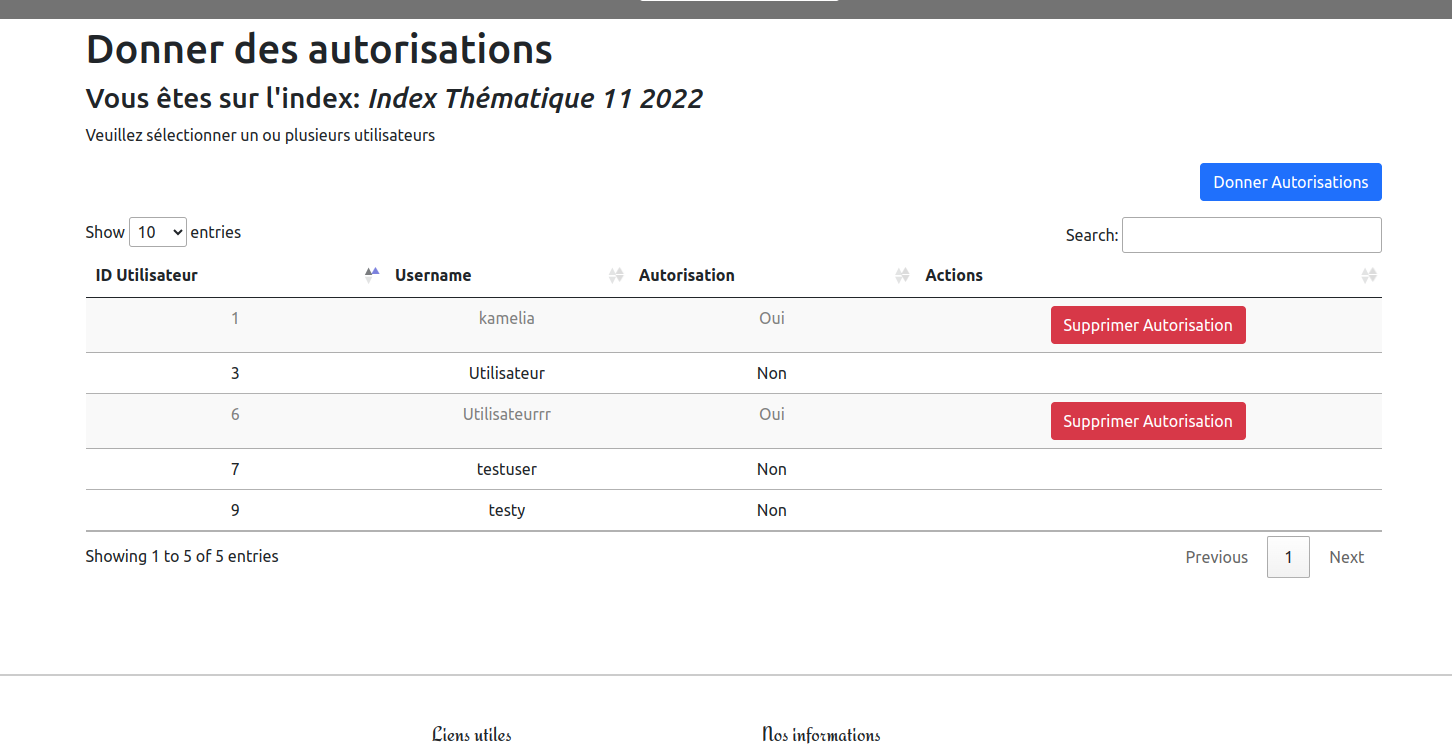
\includegraphics[width=1\textwidth]{images/Capture d’écran du 2025-02-08 21-20-34.png} 
    \caption{Gestion des Autorisations sur les Index}
    \label{fig:gestion_autorisations_index}
\end{figure}
\begin{figure}[h]
    \centering
    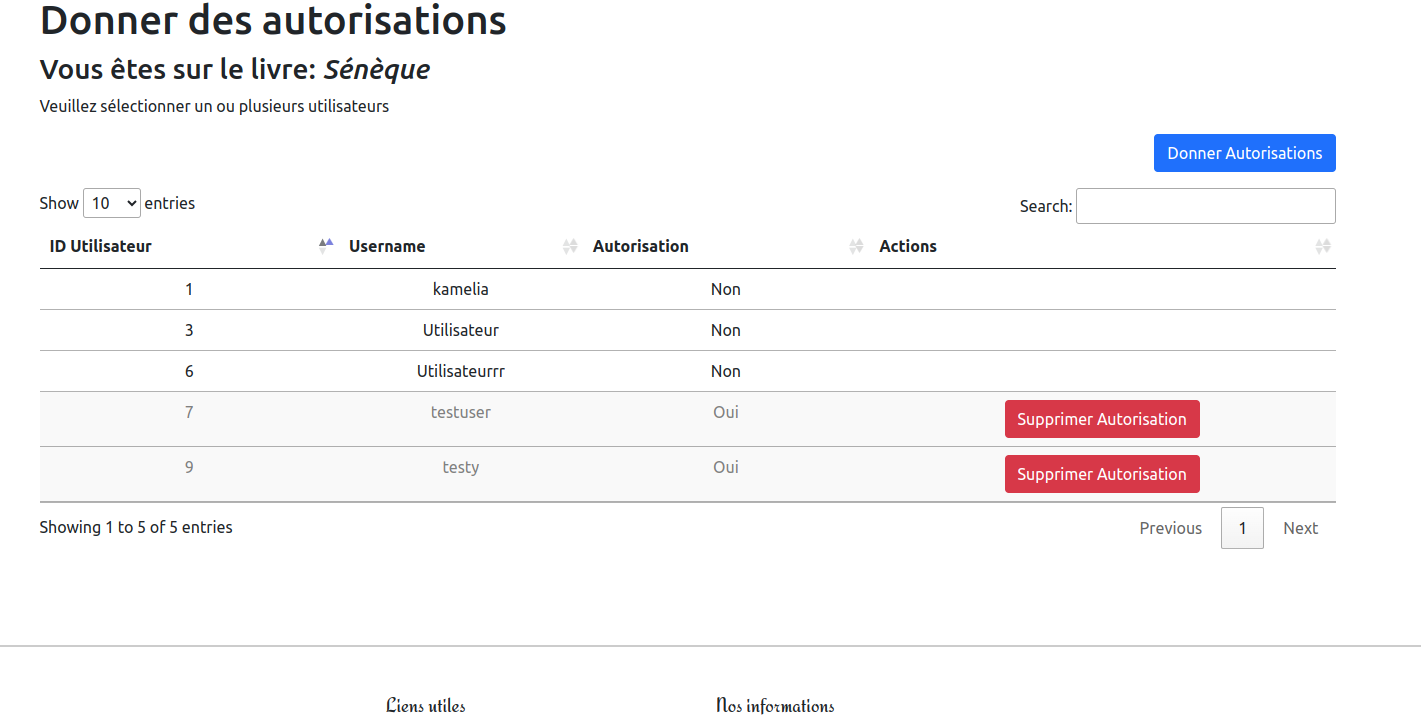
\includegraphics[width=1.1\textwidth]{images/Capture d’écran du 2025-02-08 21-23-25.png} 
    \caption{Gestion des Autorisations sur les Livres}
    \label{fig:gestion_autorisations_livre}
\end{figure}
\begin{figure}[h]
    \centering
    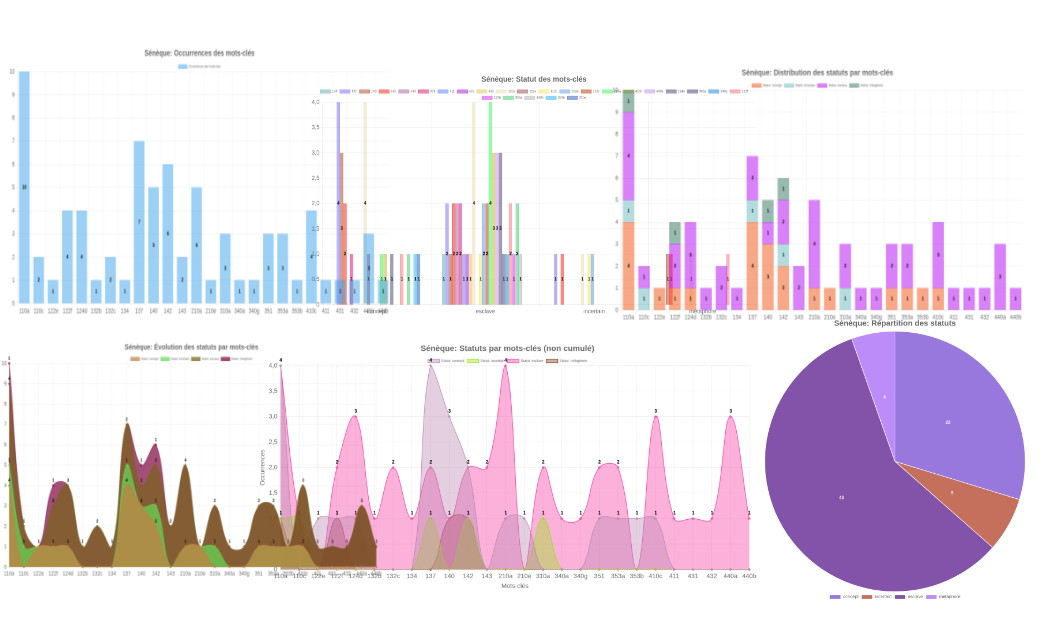
\includegraphics[width=1.1\textwidth]{images/Capture d’écran du 2025-02-12 13-37-42.png} 
    \caption{Aperçu des six graphiques}
    \label{fig:graphes}
\end{figure}
\begin{figure}[h]
    \centering
    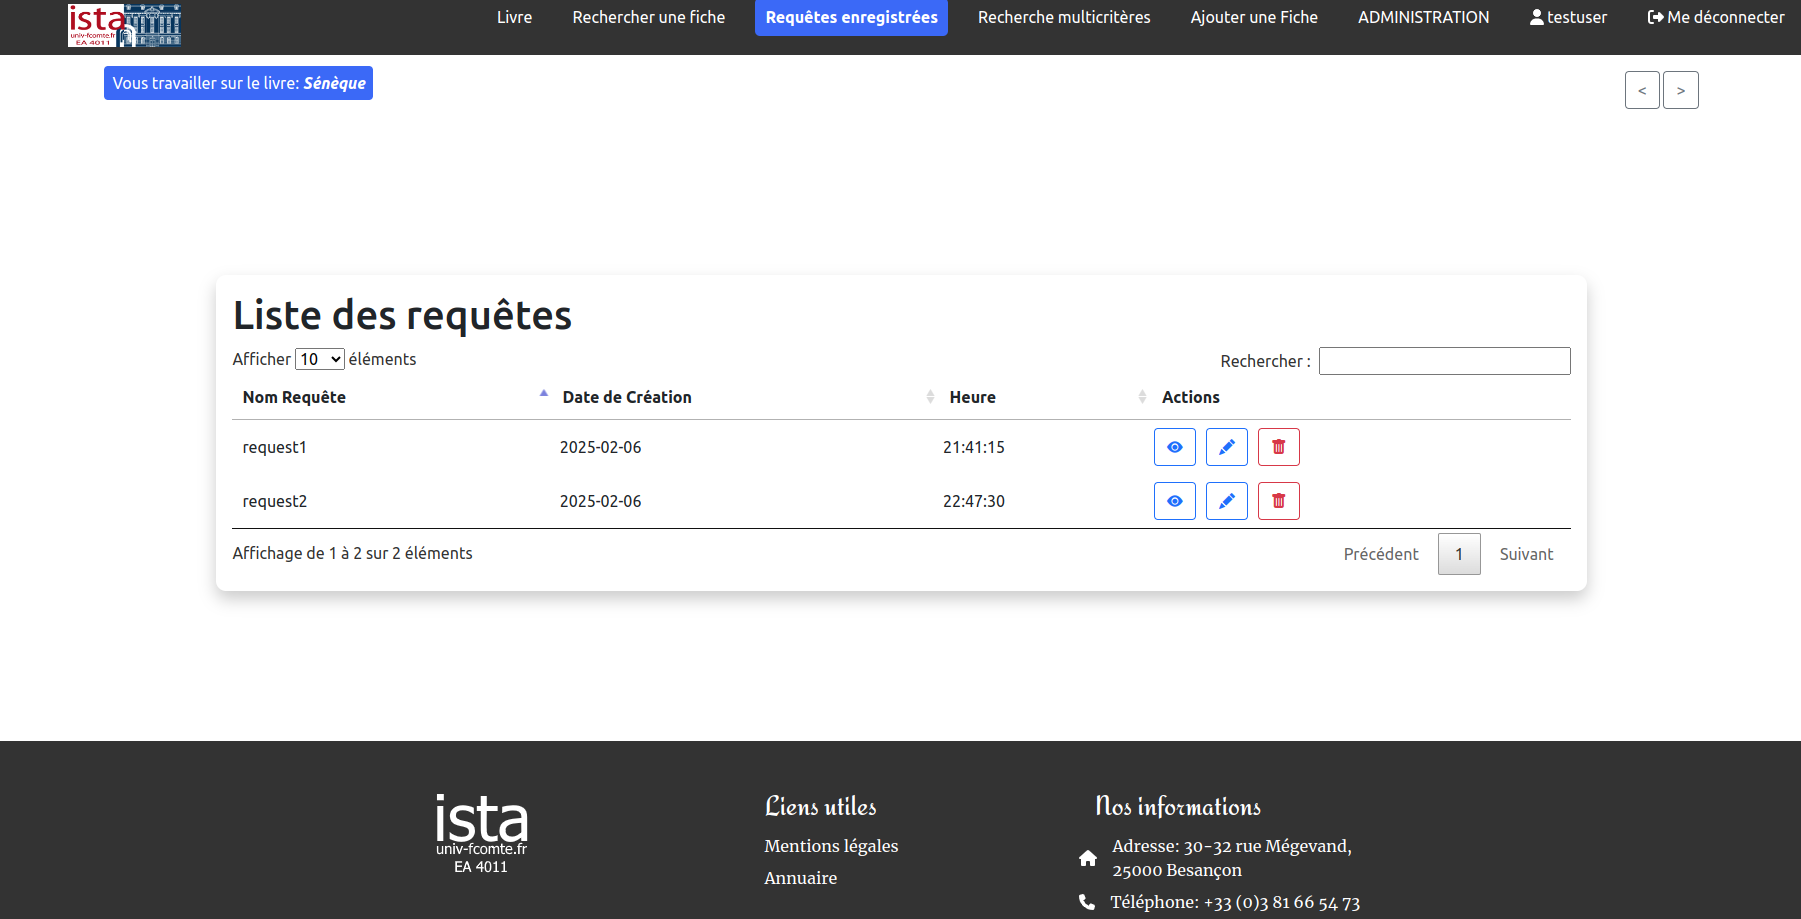
\includegraphics[width=1.1\textwidth]{images/sav_req.png} 
    \caption{Gestion des requêtes enregistrées}
    \label{fig:gestion_sav_req}
\end{figure}
\begin{figure}[h]
    \centering
    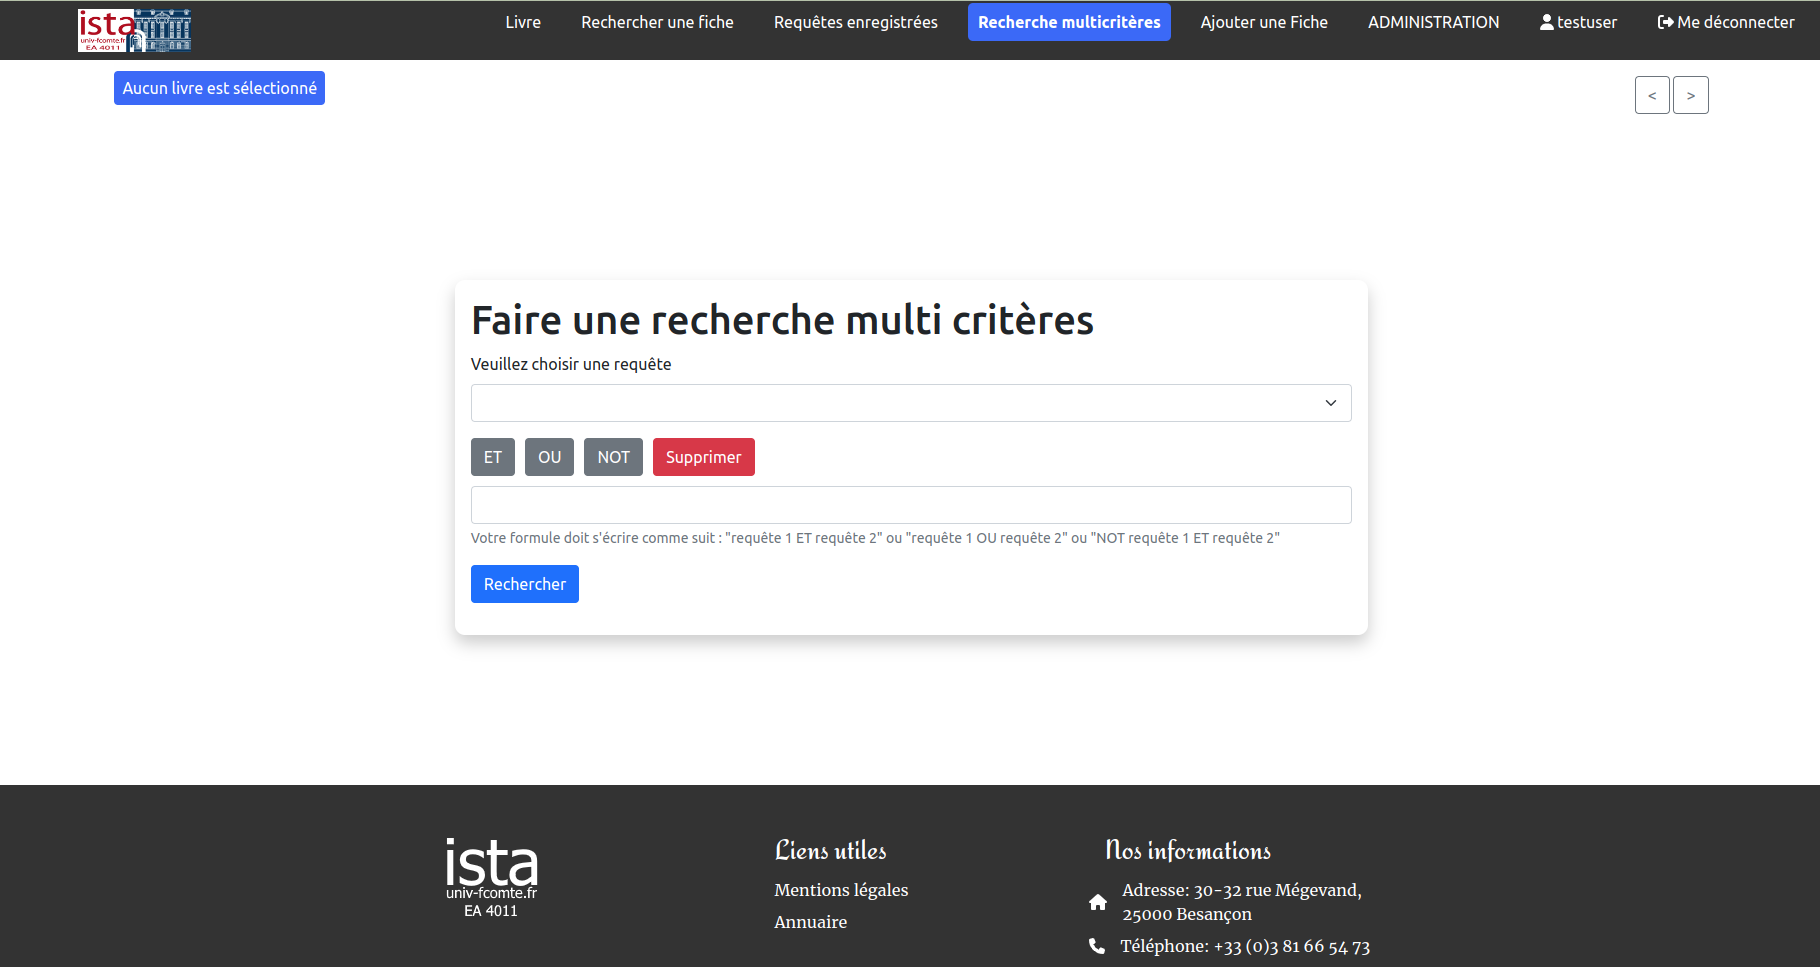
\includegraphics[width=1.1\textwidth]{images/rech_multi_crit.png} 
    \caption{Recherche multicritères}
    \label{fig:recherche_multi}
\end{figure}
\begin{figure}[h]
    \centering
    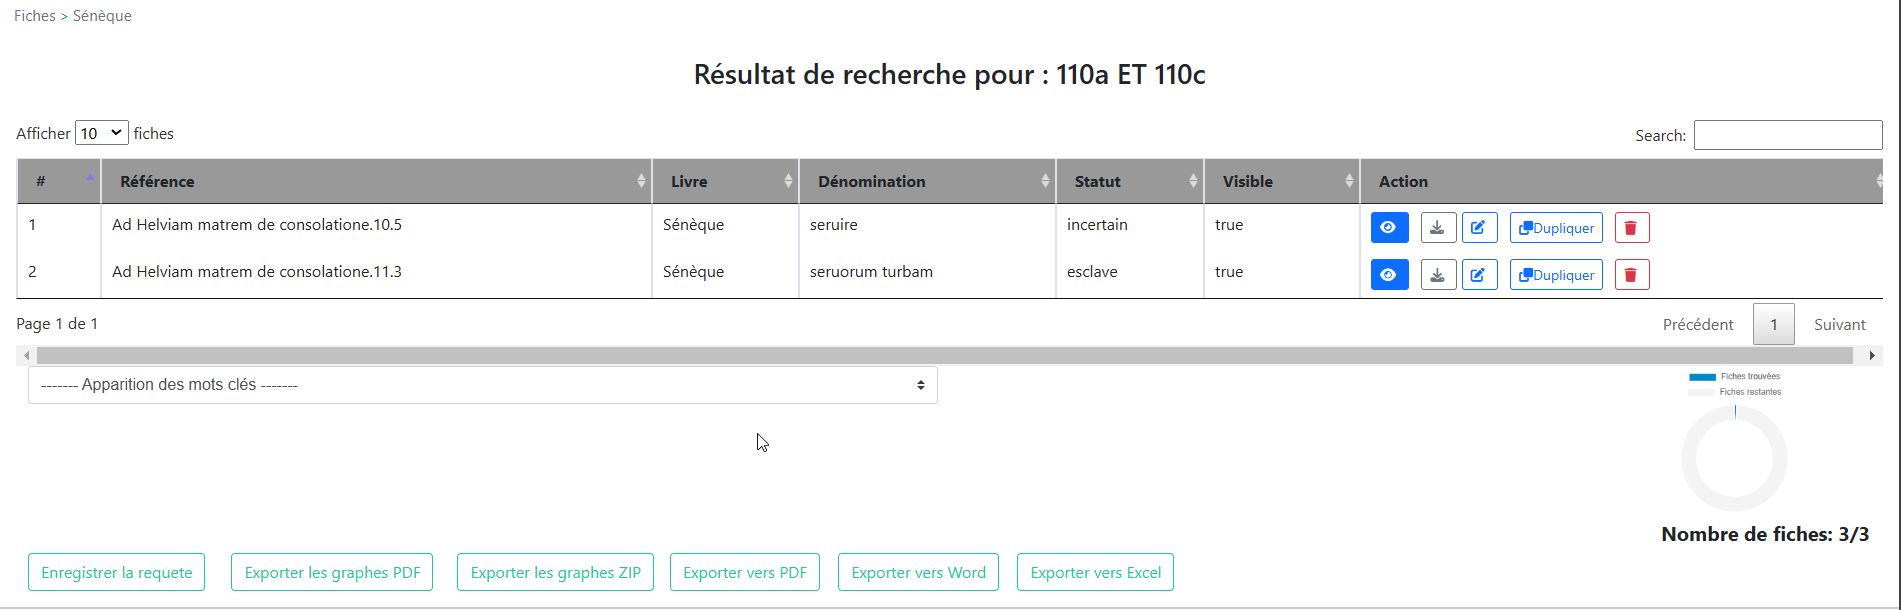
\includegraphics[width=1.1\textwidth]{images/res_rech.png} 
    \caption{Résultats de recherche}
    \label{fig:recherche_res}
\end{figure}
\begin{figure}[h]
    \centering
    
\includegraphics[width=0.5\textwidth]{images/Capture d’écran du 2025-02-10 12-48-16.png} 
    \caption{Aperçu des Améliorations Apportées}
    \label{fig:style1}
\end{figure}
\begin{figure}[h]
    \centering
    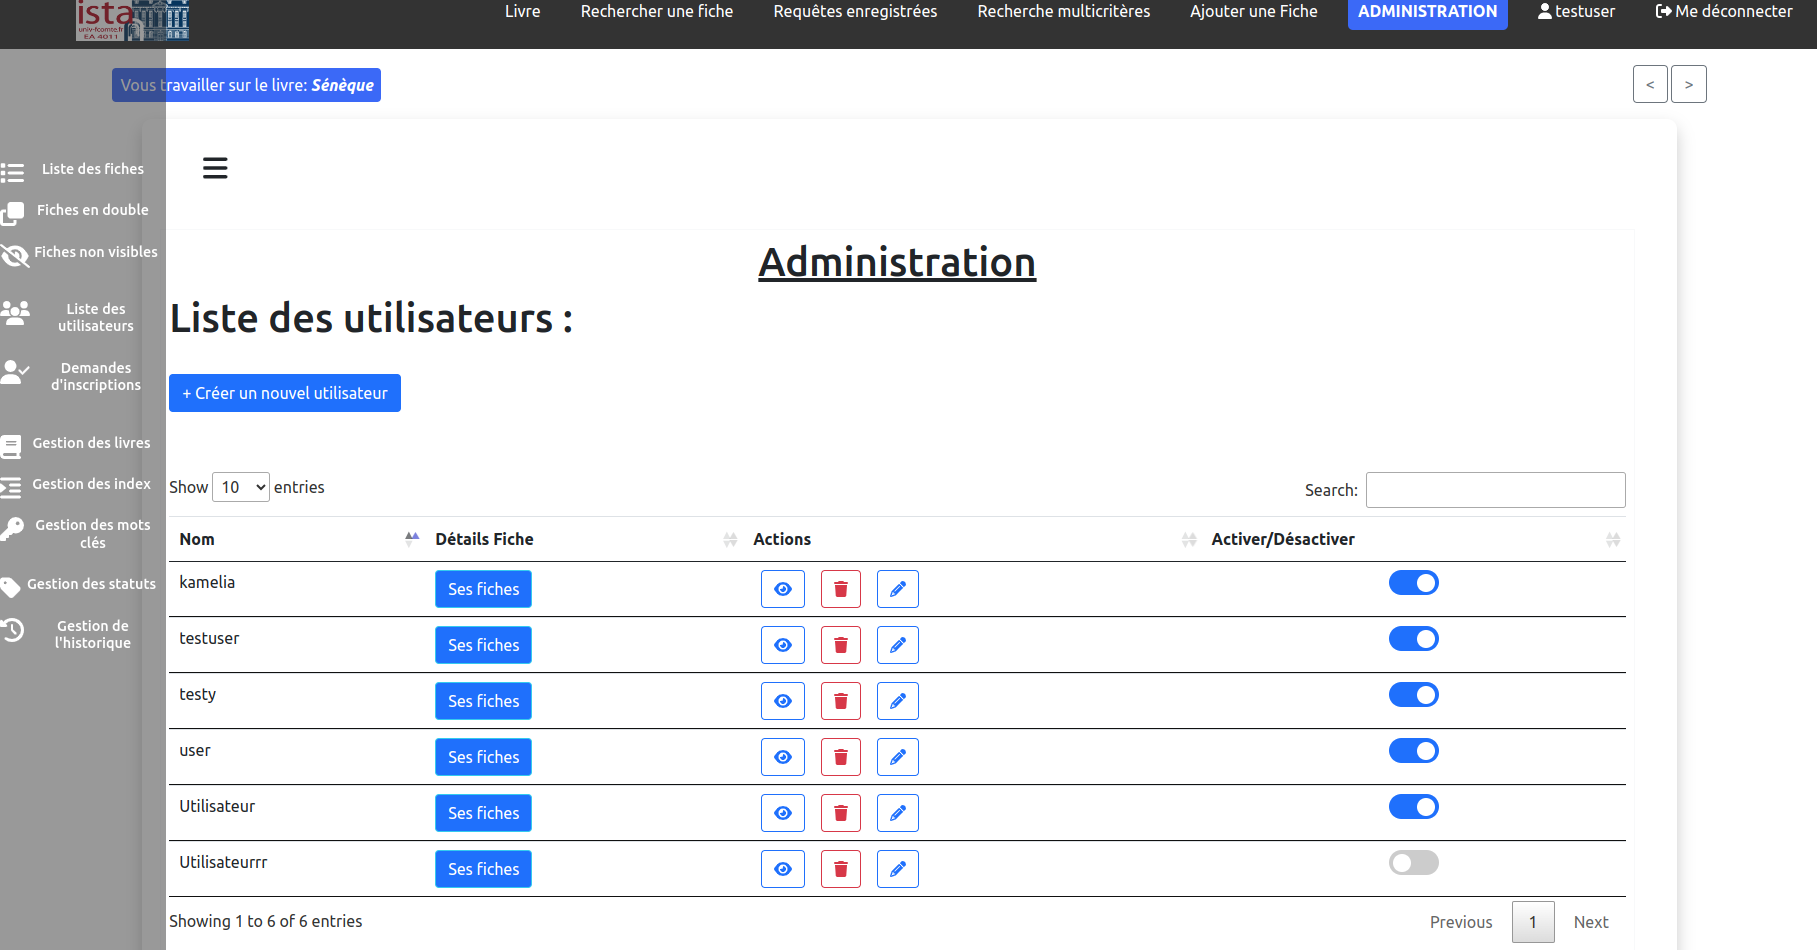
\includegraphics[width=1.1\textwidth]{images/Capture d’écran du 2025-02-17 10-41-37.png} 
    \caption{Aperçu des Améliorations Apportées du Design}
    \label{fig:style2}
\end{figure}
\begin{figure}[h]
    \centering
    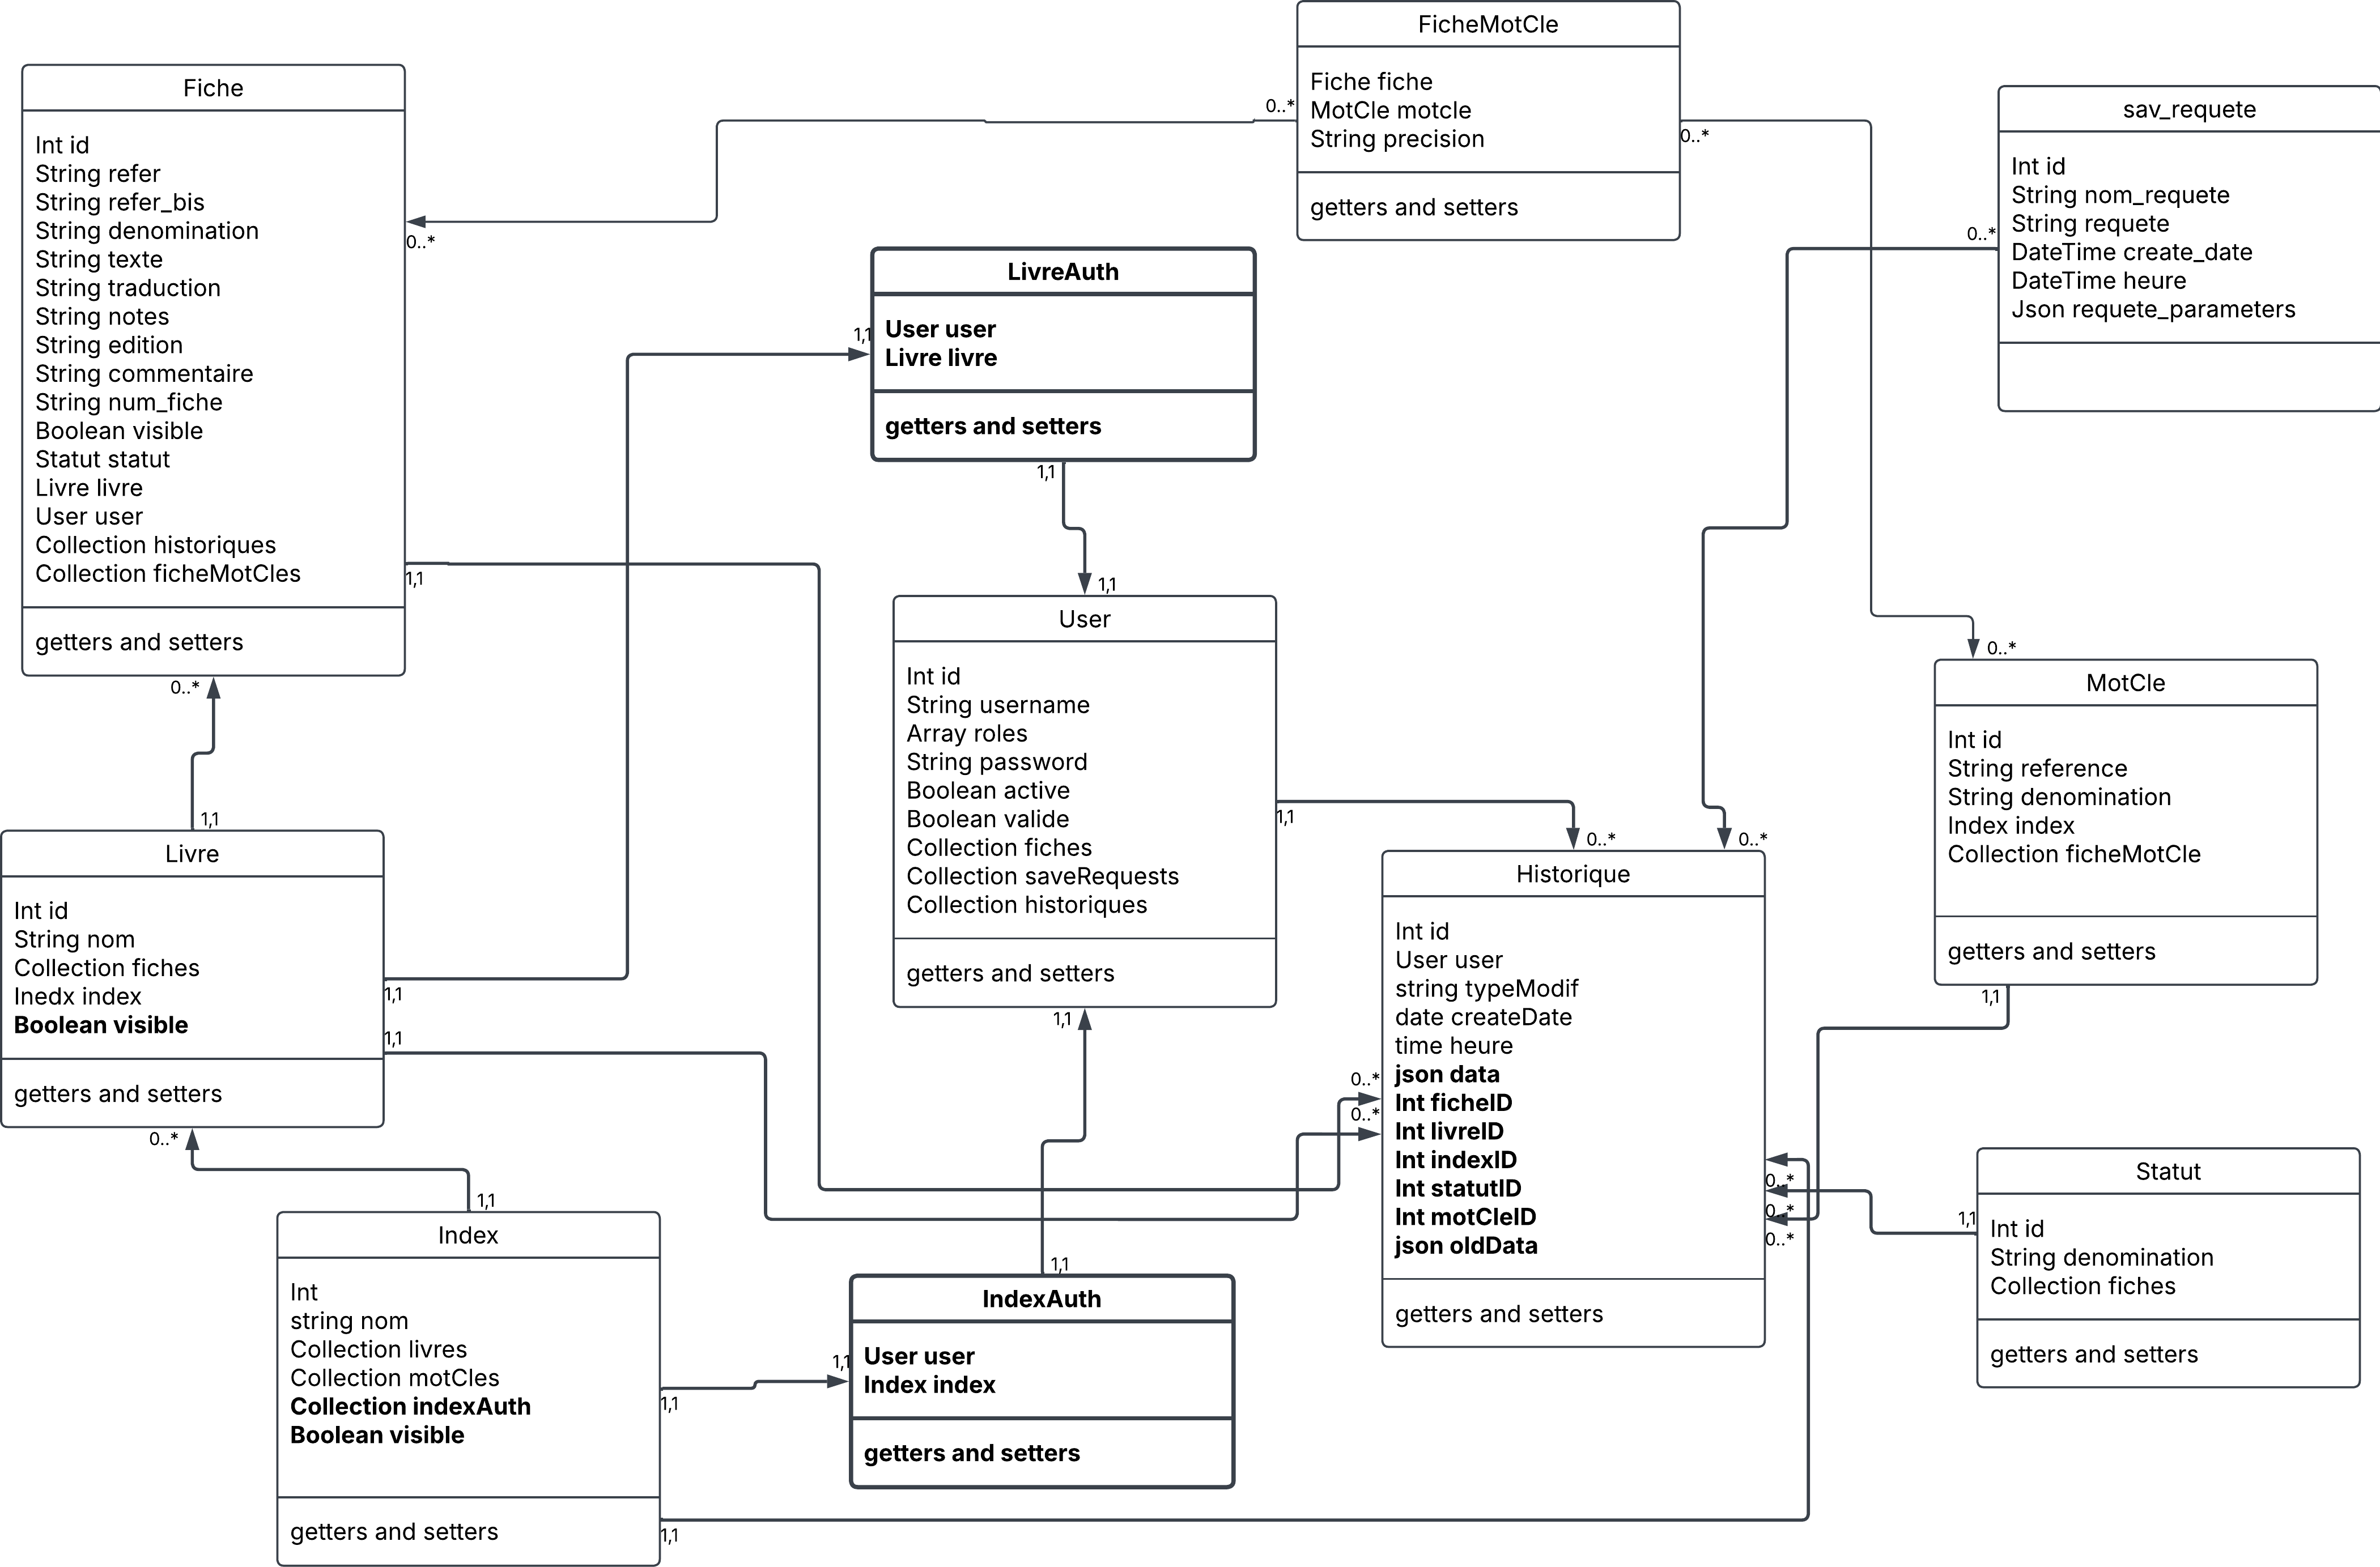
\includegraphics[width=1.1\textwidth]{images/Symfony - Page 1.png} 
    \caption{Schéma de la base de données}
    \label{fig:schema}
\end{figure}
\clearpage
\section{Bibliographie}
\begin{itemize}
        \item Wikipedia - Symfony. Disponible sur :
        \url{https://fr.wikipedia.org/wiki/Symfony} (Consulté le 28/01/2025)
    En plus de ces évolutions fonctionnelles, nous avons corrigé plusieurs bugs, optimisé le code existant et amélioré l'organisation générale de l'application. Ce projet a ainsi permis de proposer une plateforme plus performante, mieux adaptée aux besoins des utilisateurs et prête pour de futurs développements.

    \newpage


    \section{Annexes}
    \begin{figure}[h]
        \centering
        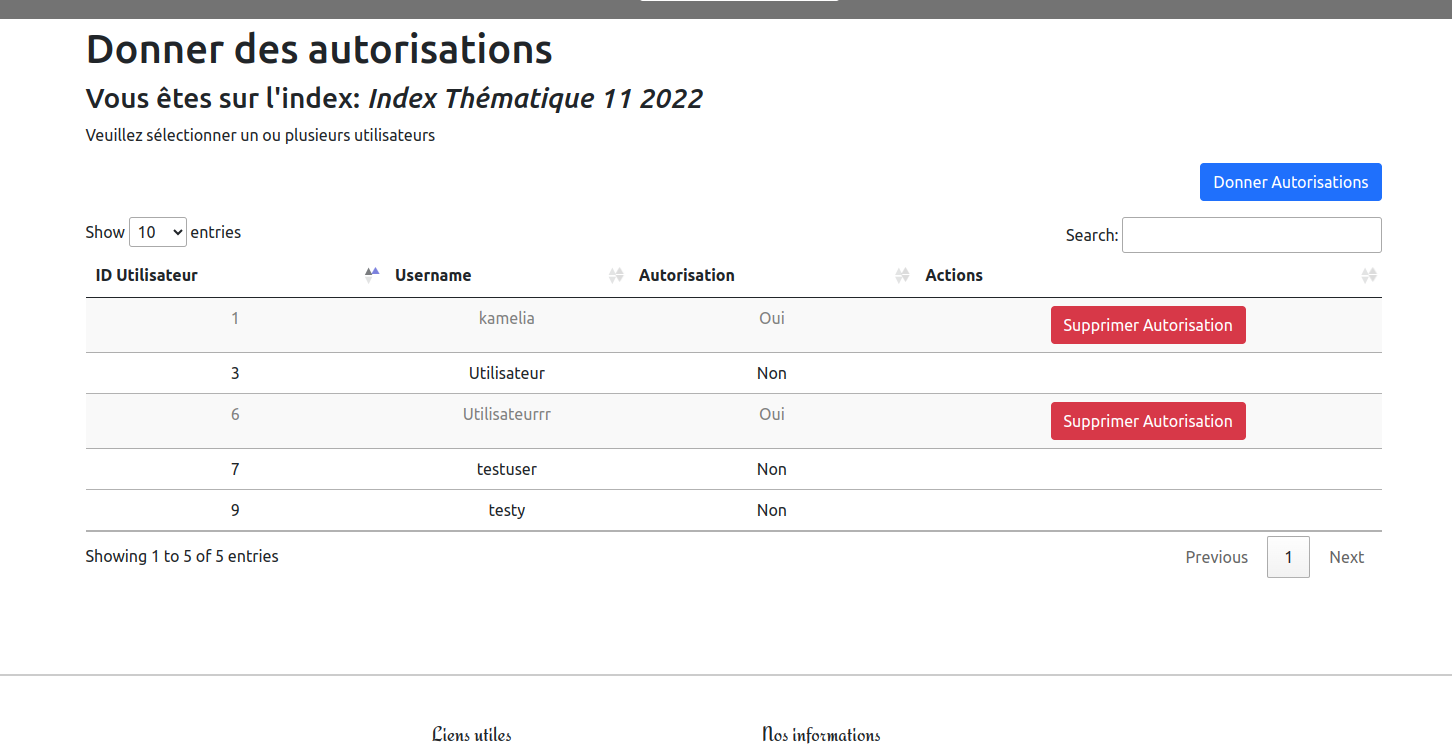
\includegraphics[width=1\textwidth]{images/Capture d’écran du 2025-02-08 21-20-34.png}
        \caption{Gestion des Autorisations sur les Index}
        \label{fig:gestion_autorisations_index}
    \end{figure}
    \begin{figure}[h]
        \centering
        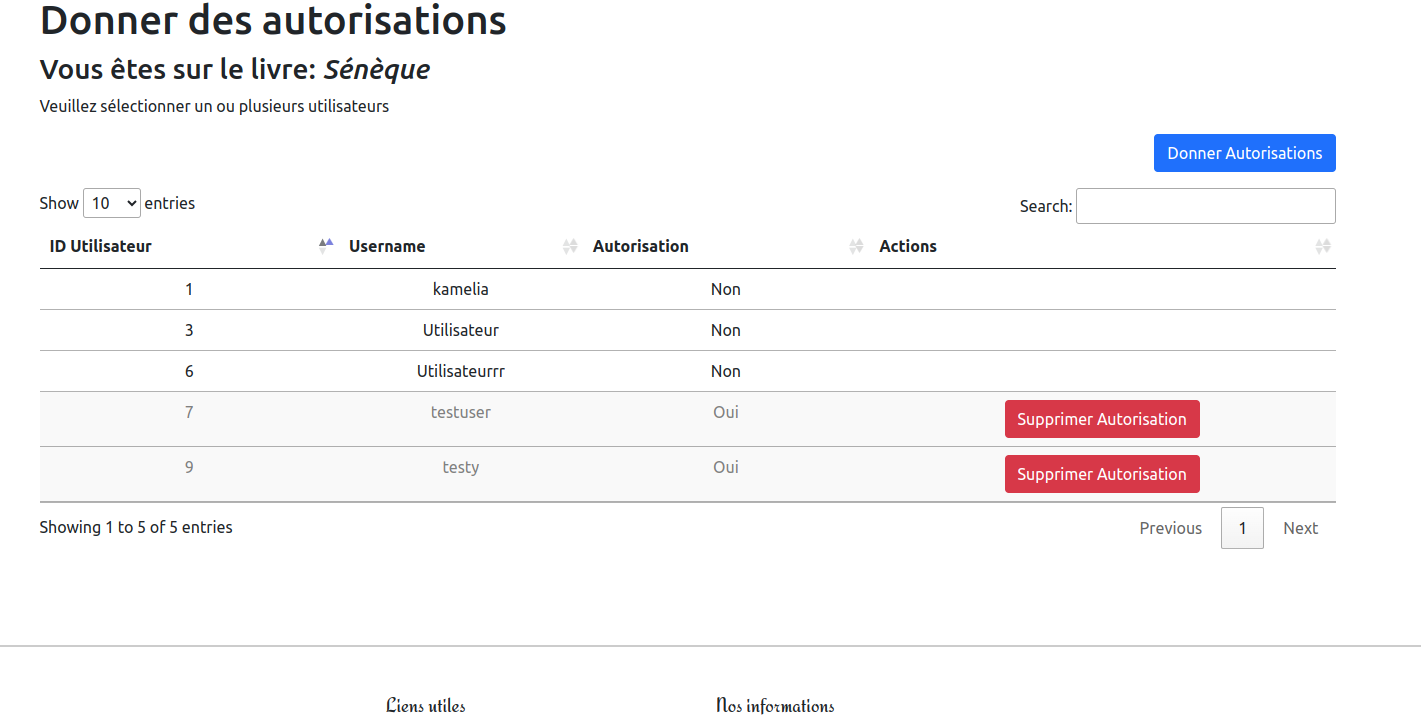
\includegraphics[width=1.1\textwidth]{images/Capture d’écran du 2025-02-08 21-23-25.png}
        \caption{Gestion des Autorisations sur les Livres}
        \label{fig:gestion_autorisations_livre}
    \end{figure}
    \begin{figure}[h]
        \centering
        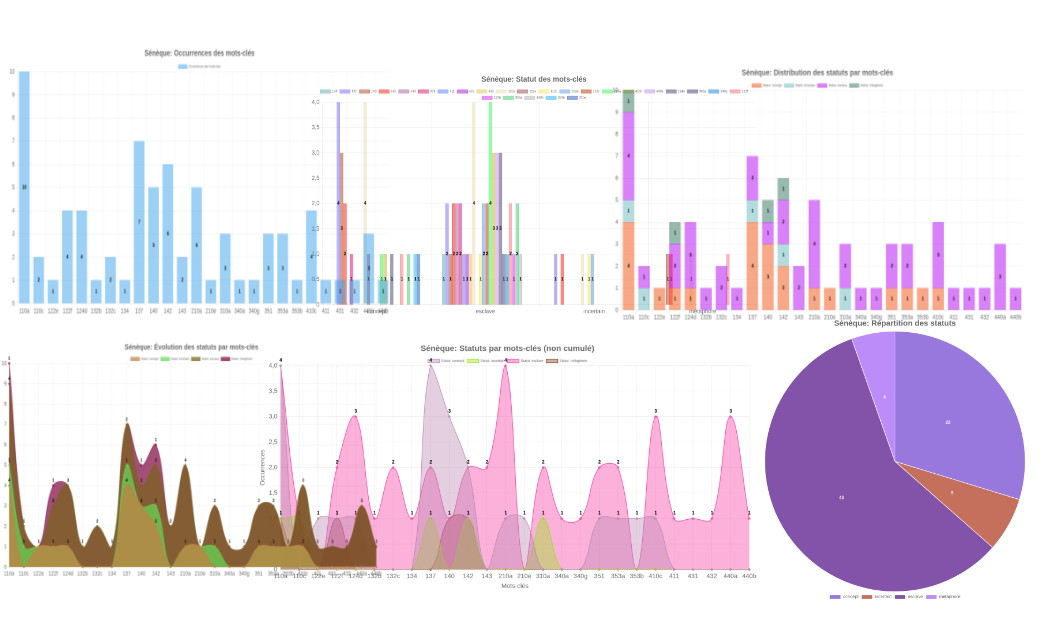
\includegraphics[width=1.1\textwidth]{images/Capture d’écran du 2025-02-12 13-37-42.png}
        \caption{Aperçu des six graphiques}
        \label{fig:graphes}
    \end{figure}
    \begin{figure}[h]
        \centering
        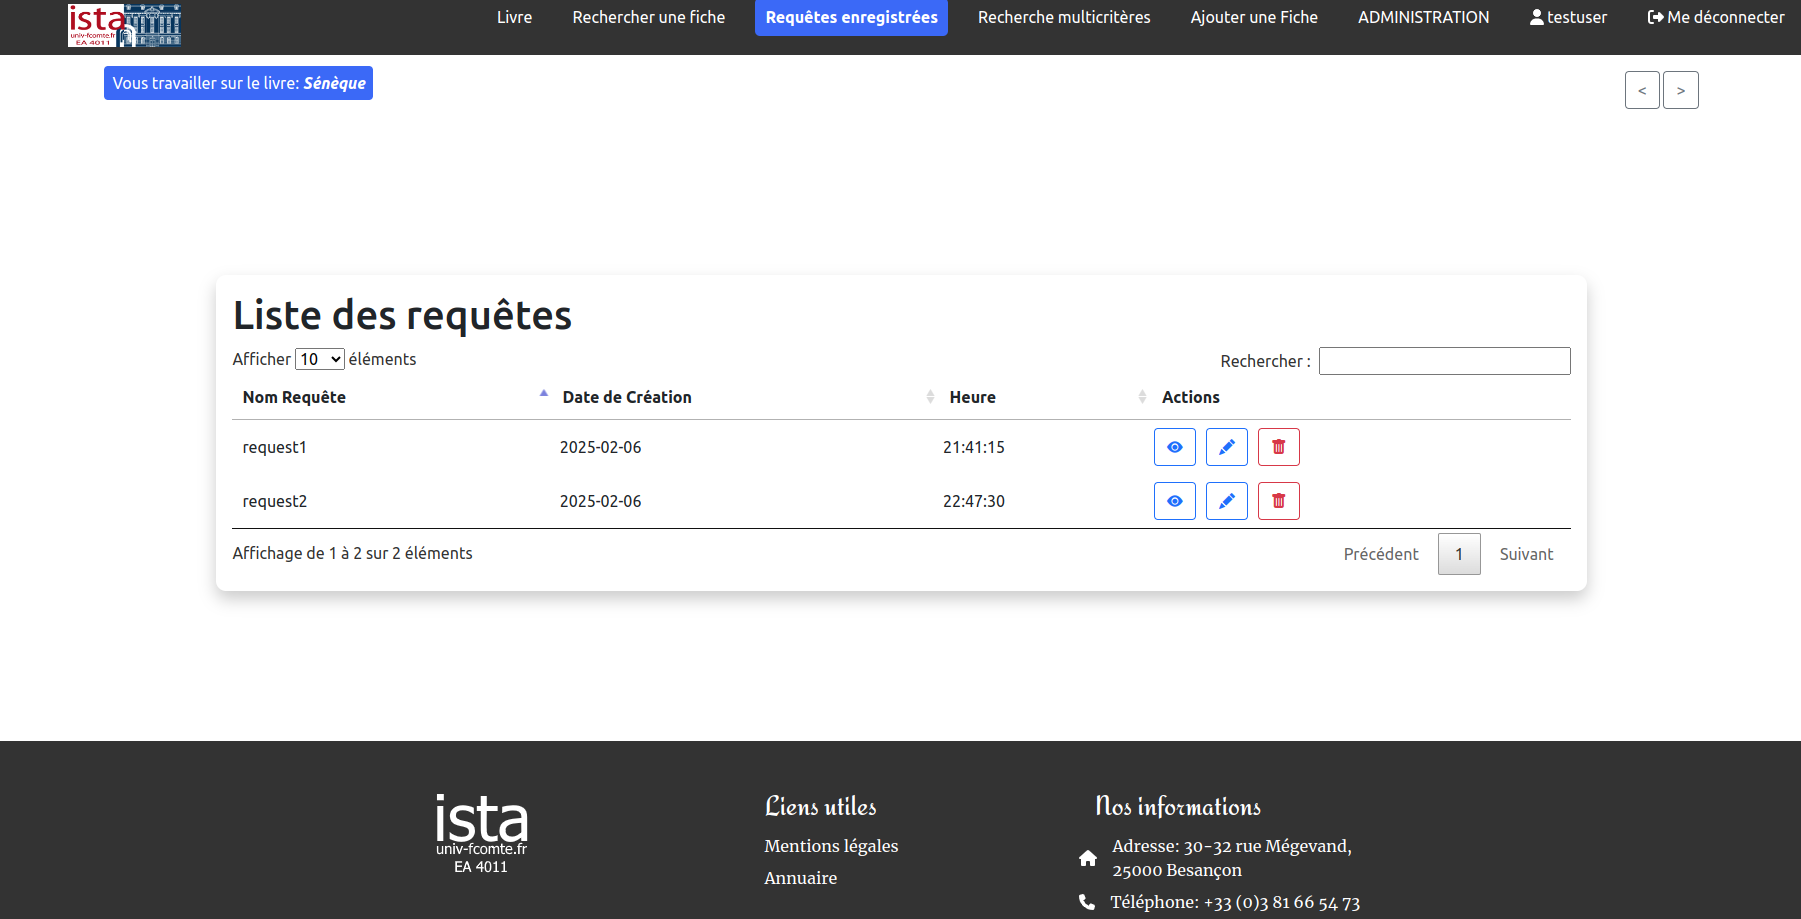
\includegraphics[width=1.1\textwidth]{images/sav_req.png}
        \caption{Gestion des requêtes enregistrées}
        \label{fig:gestion_sav_req}
    \end{figure}
    \begin{figure}[h]
        \centering
        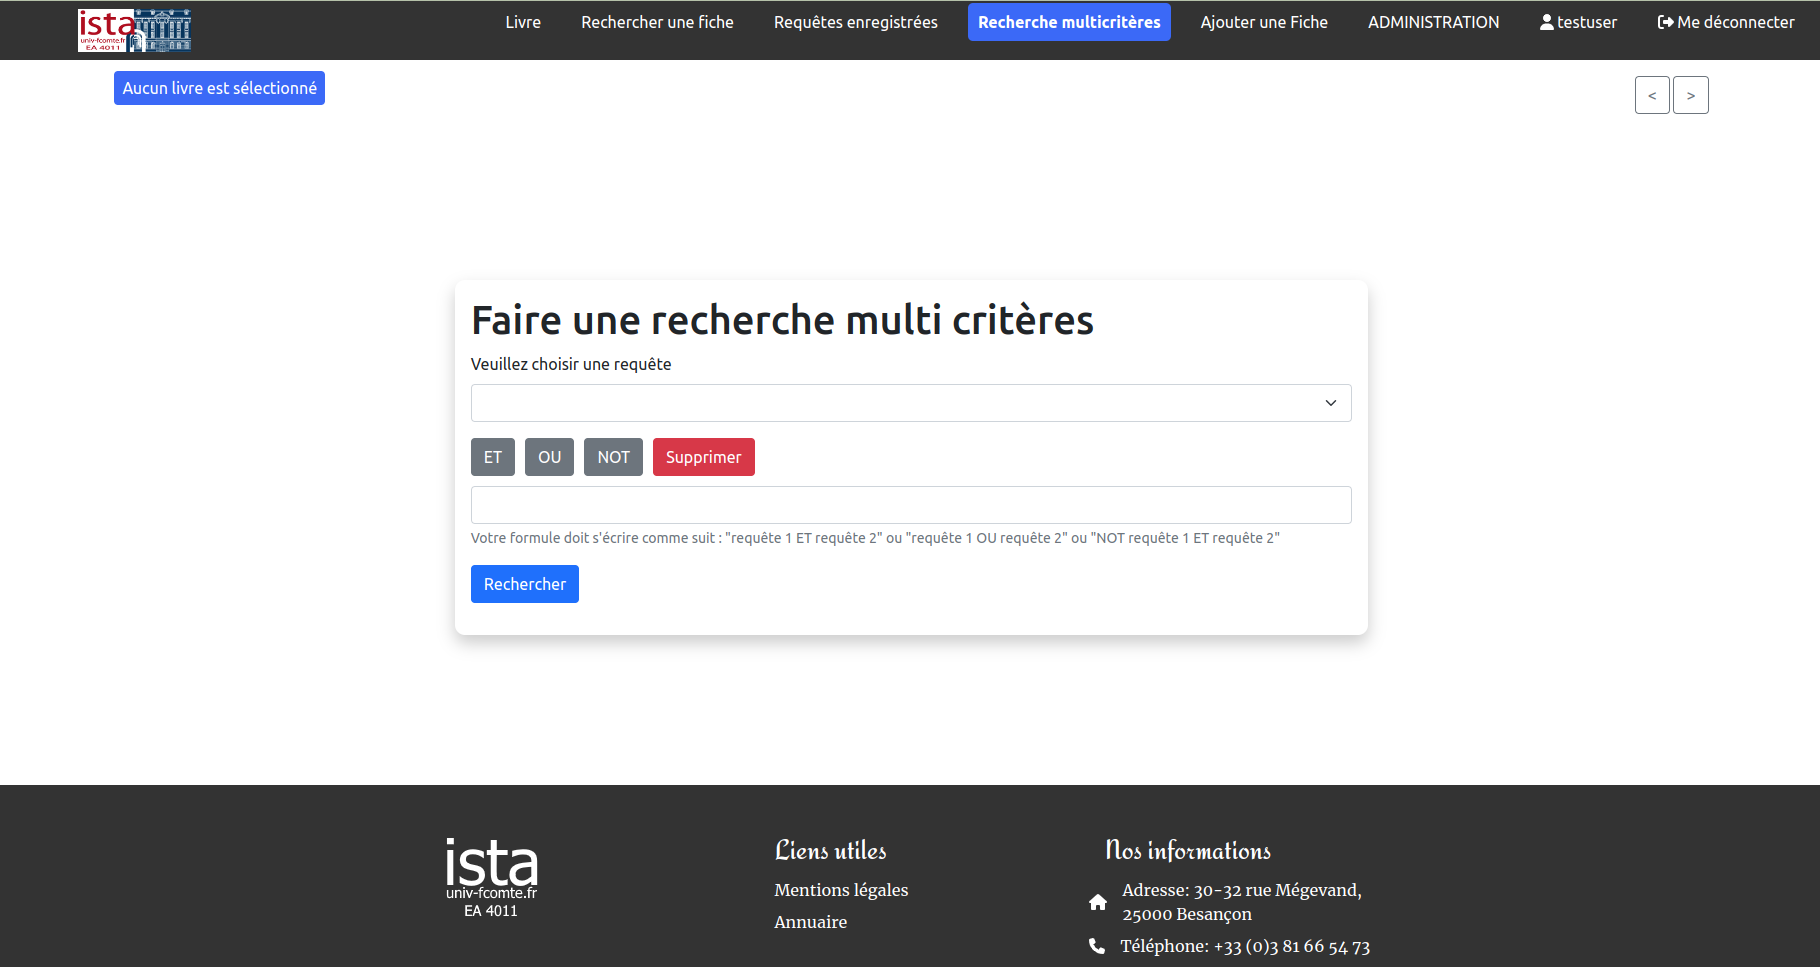
\includegraphics[width=1.1\textwidth]{images/rech_multi_crit.png}
        \caption{Recherche multicritères}
        \label{fig:recherche_multi}
    \end{figure}
    \begin{figure}[h]
        \centering
        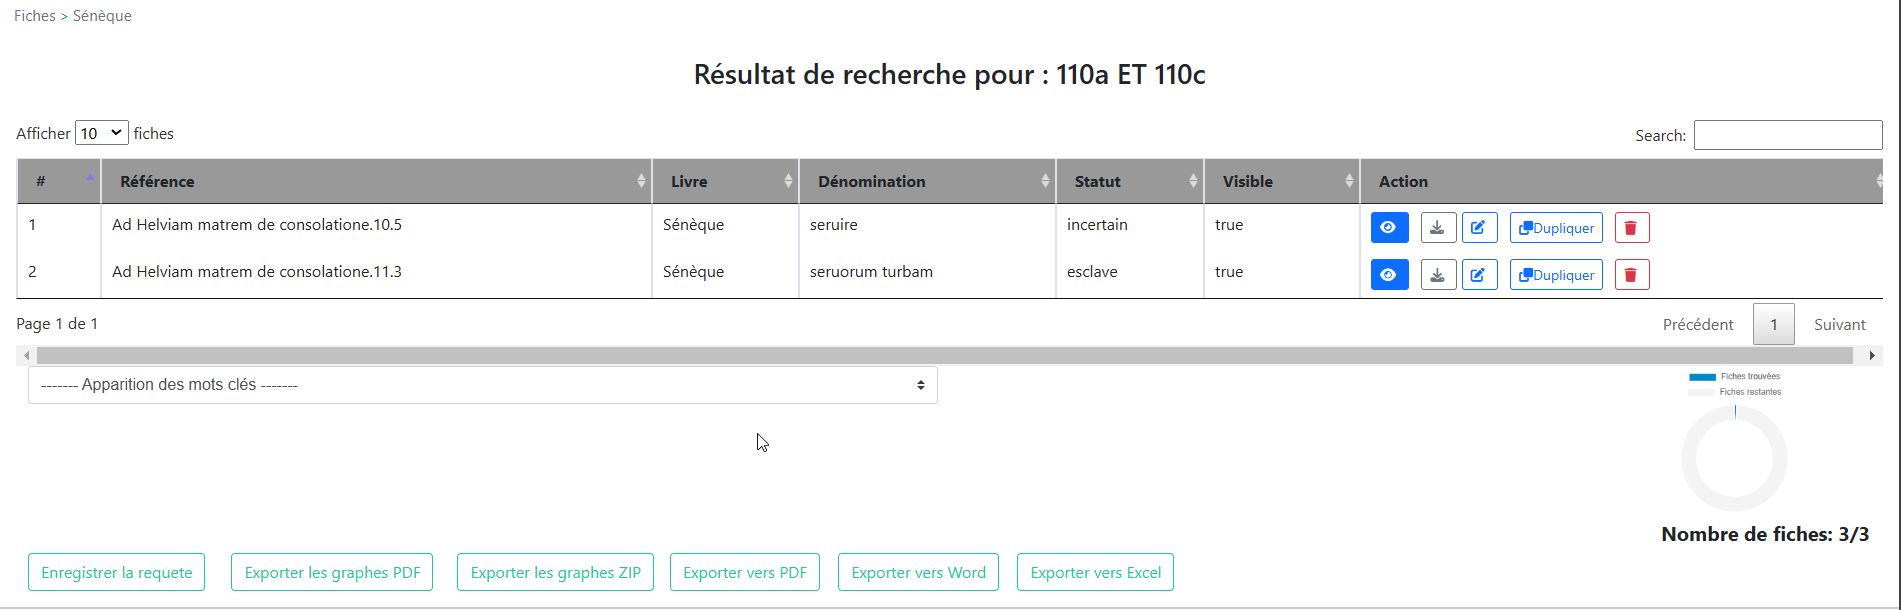
\includegraphics[width=1.1\textwidth]{images/res_rech.png}
        \caption{Résultats de recherche}
        \label{fig:recherche_res}
    \end{figure}
    \begin{figure}[h]
        \centering
        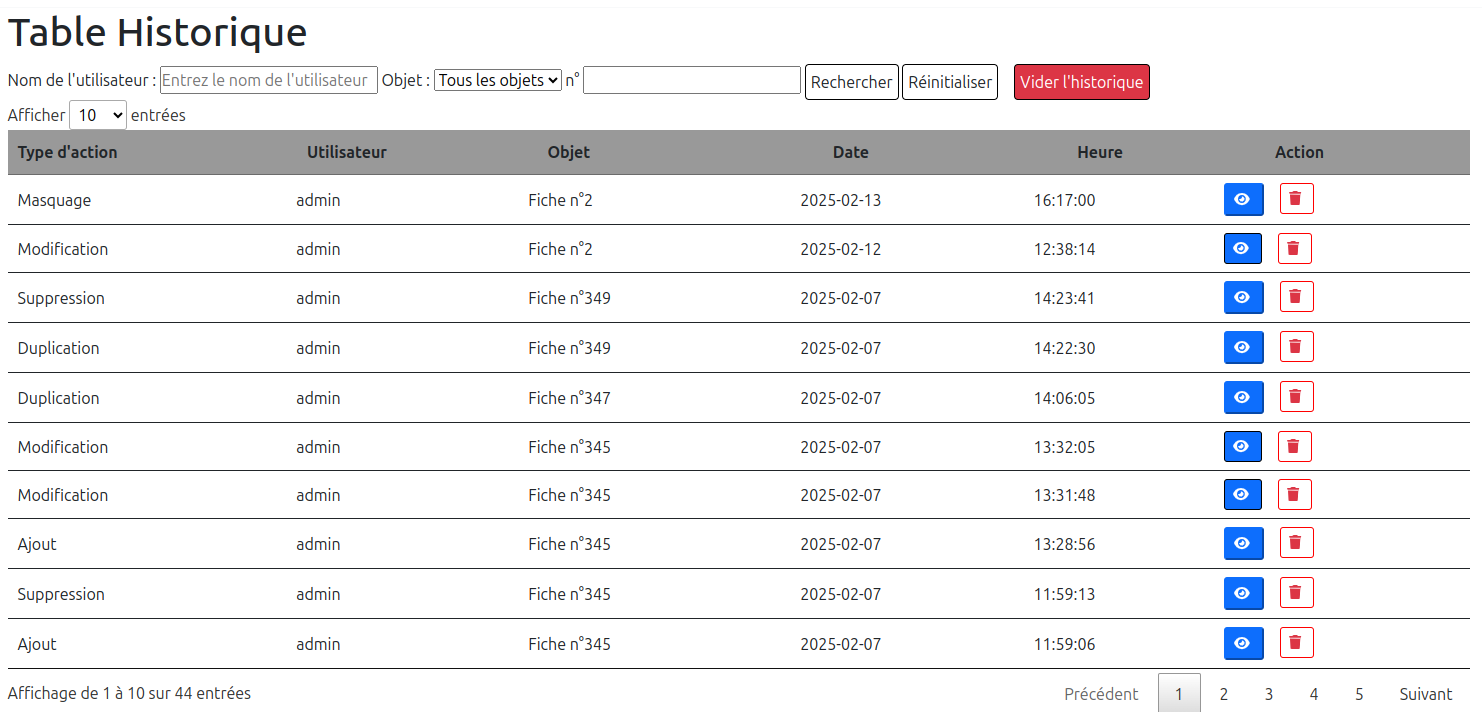
\includegraphics[width=0.5\textwidth]{images/img.png}
        \caption{Aperçu de l'historique}
        \label{fig:historique}
    \end{figure}
    \begin{figure}[h]
        \centering
        
\includegraphics[width=0.5\textwidth]{images/Capture d’écran du 2025-02-10 12-48-16.png}
        \caption{Aperçu des Améliorations Apportées}
        \label{fig:style1}
    \end{figure}
    \begin{figure}[h]
        \centering
        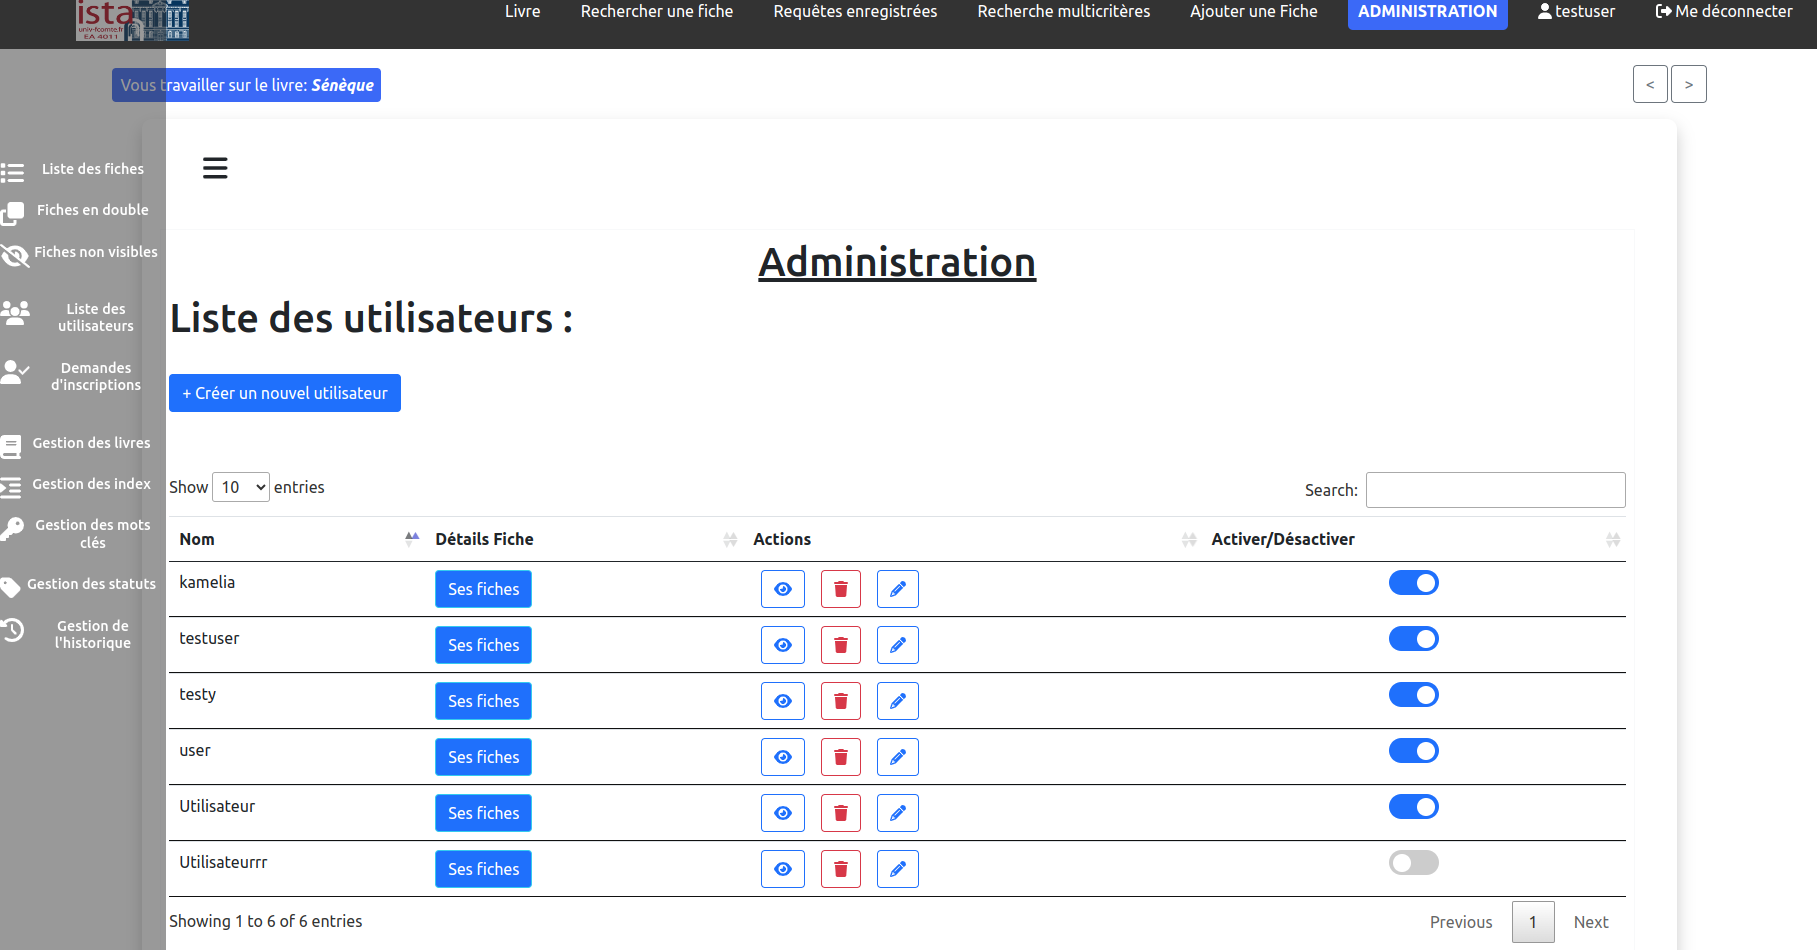
\includegraphics[width=1.1\textwidth]{images/Capture d’écran du 2025-02-17 10-41-37.png}
        \caption{Aperçu des Améliorations Apportées du Design}
        \label{fig:style2}
    \end{figure}
    \clearpage


    \section{Bibliographie}
    \begin{itemize}
        \item Wikipedia - Symfony. Disponible sur : \url{https://fr.wikipedia.org/wiki/Symfony} (Consulté le 28/01/2025)
        \item ISTA. Disponible sur : \url{https://ista.univ-fcomte.fr/} (Consulté le 15/01/2025)
        \item Symfony. Disponible sur : \url{https://symfony.com/} (Consulté le 16/02/2025)
        \item DataTables. Disponible sur : \url{https://datatables.net/} (Consulté le 04/01/2025)
        \item Bootstrap. Disponible sur : \url{https://getbootstrap.com/} (Consulté le 03/02/2025)
    \end{itemize}
\end{document}